\section{MALLM Framework} \label{app:framework}

We provide more thorough details about the framework used to run the experiments called MALLM (\textbf{M}ulti-\textbf{A}gent \textbf{L}arge \textbf{L}anguage \textbf{M}odels)\footnote{\url{https://github.com/Multi-Agent-LLMs/mallm}}.

\paragraph{\textbf{Automatic Persona Assignment.}}
Discussions with MALLM use task- and example-specific personas for the agents.
As manually specifying useful personas for each example is not feasible, we automatically assign personas that foster a rich discussion.
For this, we explicitly prompt another LLM (\textit{meta-llama/Meta-Llama-3.1-70B-Instruct}) to generate a diverse set of three expert personas for each example.
This yields a set of experts that represents various beliefs, opinions, and proficiency.
The prompt for the automatic persona assignment can be read in \Cref{app:prompts}.
My approach follows previous works like Solo-Performance-Prompting \citep{WangMWG23a} and Meta-Prompting \citep{SuzgunK24a}, which show that existing LLMs can be leveraged to generate and consult fitting personas on a problem automatically.
We use three agents for this study, following previous works \citep{ChenSB24a, YinSCG23a} because the structural complexity is better than with two agents while not being too complex to provide meaningful insights.
While other works have used different types of personas like personalities \citep{ShiZWW23a}, the personas generated in this work are experts related to the task and example.

\paragraph{\textbf{Discussion Paradigm.}}
To define the structure of the multi-agent discussion, we use the \textit{memory} paradigm defined by \citet{YinSCG23a}.
\Cref{fig:problem_drift} shows the format graphically.
With the memory paradigm, all agents contribute to the discussion once per turn and have all the information available.
While there are potentially many ways to define the discourse's structure, we choose this paradigm because of its simplicity, keeping the human assessment of agent discussions manageable.

\paragraph{\textbf{Voting.}}
A voting mechanism at the end of each turn allows for a fixed discussion length while still providing a solution to evaluate at each turn.
We select this iterative voting approach because it universally fits our diverse selection of generative and QA tasks.
The prompt for the voting is visible in \Cref{app:prompts}.
In the case that the agents produce a tie by voting, we select a random one.
This only happened with 0.65\% of all voting procedures.
Using voting, this study differs from other works that either employ no decision-making at all \citep{SchickDJP22a} or use a judge agent that makes the final decision \citep{SunYLW24}.
Meanwhile, this voting approach yields a definitive solution to evaluate after each turn.

\section{Parameters} \label{app:parameters}

We adhere to default parameters for our used models, using langchain 0.1.16 and openai 1.25.0 for the implementation of the MALLM framework.

\begin{itemize}[noitemsep]%
    \item \texttt{temperature = 1.0}
    \item \texttt{top\_p = 1.0}
    \item \texttt{presence\_penalty = 0.0}
    \item \texttt{frequency\_penalty = 0.0}
    \item \texttt{max\_tokens = 1024}
\end{itemize}

\section{Prompts} \label{app:prompts}

\section{Discussion of Assumptions}\label{sec:discussion}
In this paper, we have made several assumptions for the sake of clarity and simplicity. In this section, we discuss the rationale behind these assumptions, the extent to which these assumptions hold in practice, and the consequences for our protocol when these assumptions hold.

\subsection{Assumptions on the Demand}

There are two simplifying assumptions we make about the demand. First, we assume the demand at any time is relatively small compared to the channel capacities. Second, we take the demand to be constant over time. We elaborate upon both these points below.

\paragraph{Small demands} The assumption that demands are small relative to channel capacities is made precise in \eqref{eq:large_capacity_assumption}. This assumption simplifies two major aspects of our protocol. First, it largely removes congestion from consideration. In \eqref{eq:primal_problem}, there is no constraint ensuring that total flow in both directions stays below capacity--this is always met. Consequently, there is no Lagrange multiplier for congestion and no congestion pricing; only imbalance penalties apply. In contrast, protocols in \cite{sivaraman2020high, varma2021throughput, wang2024fence} include congestion fees due to explicit congestion constraints. Second, the bound \eqref{eq:large_capacity_assumption} ensures that as long as channels remain balanced, the network can always meet demand, no matter how the demand is routed. Since channels can rebalance when necessary, they never drop transactions. This allows prices and flows to adjust as per the equations in \eqref{eq:algorithm}, which makes it easier to prove the protocol's convergence guarantees. This also preserves the key property that a channel's price remains proportional to net money flow through it.

In practice, payment channel networks are used most often for micro-payments, for which on-chain transactions are prohibitively expensive; large transactions typically take place directly on the blockchain. For example, according to \cite{river2023lightning}, the average channel capacity is roughly $0.1$ BTC ($5,000$ BTC distributed over $50,000$ channels), while the average transaction amount is less than $0.0004$ BTC ($44.7k$ satoshis). Thus, the small demand assumption is not too unrealistic. Additionally, the occasional large transaction can be treated as a sequence of smaller transactions by breaking it into packets and executing each packet serially (as done by \cite{sivaraman2020high}).
Lastly, a good path discovery process that favors large capacity channels over small capacity ones can help ensure that the bound in \eqref{eq:large_capacity_assumption} holds.

\paragraph{Constant demands} 
In this work, we assume that any transacting pair of nodes have a steady transaction demand between them (see Section \ref{sec:transaction_requests}). Making this assumption is necessary to obtain the kind of guarantees that we have presented in this paper. Unless the demand is steady, it is unreasonable to expect that the flows converge to a steady value. Weaker assumptions on the demand lead to weaker guarantees. For example, with the more general setting of stochastic, but i.i.d. demand between any two nodes, \cite{varma2021throughput} shows that the channel queue lengths are bounded in expectation. If the demand can be arbitrary, then it is very hard to get any meaningful performance guarantees; \cite{wang2024fence} shows that even for a single bidirectional channel, the competitive ratio is infinite. Indeed, because a PCN is a decentralized system and decisions must be made based on local information alone, it is difficult for the network to find the optimal detailed balance flow at every time step with a time-varying demand.  With a steady demand, the network can discover the optimal flows in a reasonably short time, as our work shows.

We view the constant demand assumption as an approximation for a more general demand process that could be piece-wise constant, stochastic, or both (see simulations in Figure \ref{fig:five_nodes_variable_demand}).
We believe it should be possible to merge ideas from our work and \cite{varma2021throughput} to provide guarantees in a setting with random demands with arbitrary means. We leave this for future work. In addition, our work suggests that a reasonable method of handling stochastic demands is to queue the transaction requests \textit{at the source node} itself. This queuing action should be viewed in conjunction with flow-control. Indeed, a temporarily high unidirectional demand would raise prices for the sender, incentivizing the sender to stop sending the transactions. If the sender queues the transactions, they can send them later when prices drop. This form of queuing does not require any overhaul of the basic PCN infrastructure and is therefore simpler to implement than per-channel queues as suggested by \cite{sivaraman2020high} and \cite{varma2021throughput}.

\subsection{The Incentive of Channels}
The actions of the channels as prescribed by the DEBT control protocol can be summarized as follows. Channels adjust their prices in proportion to the net flow through them. They rebalance themselves whenever necessary and execute any transaction request that has been made of them. We discuss both these aspects below.

\paragraph{On Prices}
In this work, the exclusive role of channel prices is to ensure that the flows through each channel remains balanced. In practice, it would be important to include other components in a channel's price/fee as well: a congestion price  and an incentive price. The congestion price, as suggested by \cite{varma2021throughput}, would depend on the total flow of transactions through the channel, and would incentivize nodes to balance the load over different paths. The incentive price, which is commonly used in practice \cite{river2023lightning}, is necessary to provide channels with an incentive to serve as an intermediary for different channels. In practice, we expect both these components to be smaller than the imbalance price. Consequently, we expect the behavior of our protocol to be similar to our theoretical results even with these additional prices.

A key aspect of our protocol is that channel fees are allowed to be negative. Although the original Lightning network whitepaper \cite{poon2016bitcoin} suggests that negative channel prices may be a good solution to promote rebalancing, the idea of negative prices in not very popular in the literature. To our knowledge, the only prior work with this feature is \cite{varma2021throughput}. Indeed, in papers such as \cite{van2021merchant} and \cite{wang2024fence}, the price function is explicitly modified such that the channel price is never negative. The results of our paper show the benefits of negative prices. For one, in steady state, equal flows in both directions ensure that a channel doesn't loose any money (the other price components mentioned above ensure that the channel will only gain money). More importantly, negative prices are important to ensure that the protocol selectively stifles acyclic flows while allowing circulations to flow. Indeed, in the example of Section \ref{sec:flow_control_example}, the flows between nodes $A$ and $C$ are left on only because the large positive price over one channel is canceled by the corresponding negative price over the other channel, leading to a net zero price.

Lastly, observe that in the DEBT control protocol, the price charged by a channel does not depend on its capacity. This is a natural consequence of the price being the Lagrange multiplier for the net-zero flow constraint, which also does not depend on the channel capacity. In contrast, in many other works, the imbalance price is normalized by the channel capacity \cite{ren2018optimal, lin2020funds, wang2024fence}; this is shown to work well in practice. The rationale for such a price structure is explained well in \cite{wang2024fence}, where this fee is derived with the aim of always maintaining some balance (liquidity) at each end of every channel. This is a reasonable aim if a channel is to never rebalance itself; the experiments of the aforementioned papers are conducted in such a regime. In this work, however, we allow the channels to rebalance themselves a few times in order to settle on a detailed balance flow. This is because our focus is on the long-term steady state performance of the protocol. This difference in perspective also shows up in how the price depends on the channel imbalance. \cite{lin2020funds} and \cite{wang2024fence} advocate for strictly convex prices whereas this work and \cite{varma2021throughput} propose linear prices.

\paragraph{On Rebalancing} 
Recall that the DEBT control protocol ensures that the flows in the network converge to a detailed balance flow, which can be sustained perpetually without any rebalancing. However, during the transient phase (before convergence), channels may have to perform on-chain rebalancing a few times. Since rebalancing is an expensive operation, it is worthwhile discussing methods by which channels can reduce the extent of rebalancing. One option for the channels to reduce the extent of rebalancing is to increase their capacity; however, this comes at the cost of locking in more capital. Each channel can decide for itself the optimum amount of capital to lock in. Another option, which we discuss in Section \ref{sec:five_node}, is for channels to increase the rate $\gamma$ at which they adjust prices. 

Ultimately, whether or not it is beneficial for a channel to rebalance depends on the time-horizon under consideration. Our protocol is based on the assumption that the demand remains steady for a long period of time. If this is indeed the case, it would be worthwhile for a channel to rebalance itself as it can make up this cost through the incentive fees gained from the flow of transactions through it in steady state. If a channel chooses not to rebalance itself, however, there is a risk of being trapped in a deadlock, which is suboptimal for not only the nodes but also the channel.

\section{Conclusion}
This work presents DEBT control: a protocol for payment channel networks that uses source routing and flow control based on channel prices. The protocol is derived by posing a network utility maximization problem and analyzing its dual minimization. It is shown that under steady demands, the protocol guides the network to an optimal, sustainable point. Simulations show its robustness to demand variations. The work demonstrates that simple protocols with strong theoretical guarantees are possible for PCNs and we hope it inspires further theoretical research in this direction.
\begin{figure}[H]
\scalebox{0.5}{%
    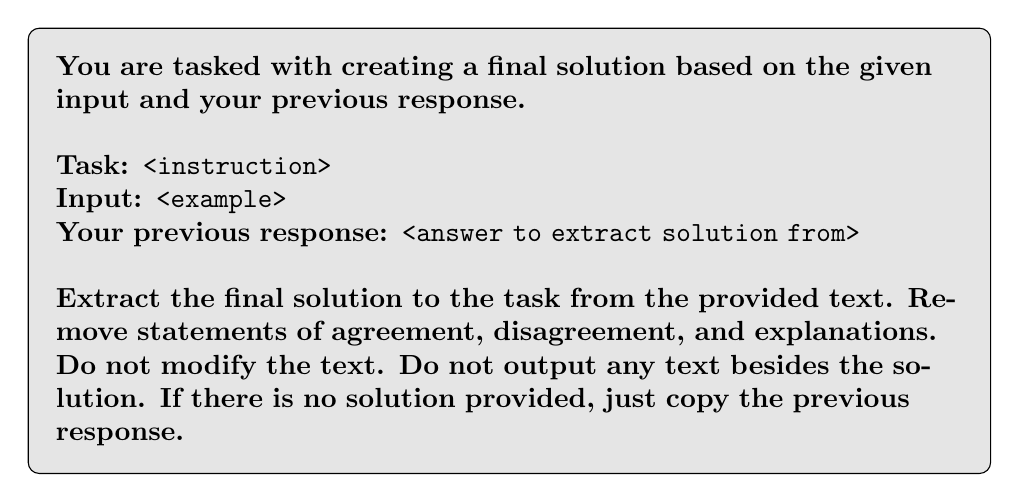
\begin{tikzpicture}
    \node [draw, rectangle, rounded corners, fill=gray!20, text width=0.95\textwidth, inner sep=10pt] (block) {
        \begin{minipage}{\textwidth}
        \textbf{You are tasked with creating a final solution based on the given input and your previous response.} \\
        
        \textbf{Task:} \texttt{<instruction>} \\
        \textbf{Input:} \texttt{<example>} \\
        \textbf{Your previous response:} \texttt{<answer to extract solution from>} \\
        
        \textbf{Extract the final solution to the task from the provided text. Remove statements of agreement, disagreement, and explanations. Do not modify the text. Do not output any text besides the solution. If there is no solution provided, just copy the previous response.}
        \end{minipage}
    };
    \end{tikzpicture}
}
\caption{Prompt to extract the solution from an agent's answer.}
\end{figure}

% \newpage
\section{Single-Winner Ranked Voting}\label{sec:single-winner-voting}
We consider $n$ voters (the agents) who need to elect one winner from a set $C$ of $m$ \emph{candidates}.
The agents' preferences are given by strict linear orderings $\succ_i$ over the candidates.

When there are only two candidates, the majority rules and its variants (weighted majority rules)  are truthful.
With three or more candidates, the   Gibbard--Satterthwaite Theorem implies that the only truthful rules are dictatorships. 
Our goal is to find non-dictatorial rules with a high RAT-degree.

%\eden{if we have time: maybe to change 'Alice' to 'voter $v_1$'} \erel{I think ``agent'' is better as it is more consistent with the rest of the paper.}

Throughout the analysis, we consider a specific agent Alice, who looks for a safe profitable manipulation. Her true ranking is $c_m \succ_A \cdots \succ_A c_1$.
We assume that, for any $j>i$, Alice strictly prefers a victory of $c_j$ to a tie between $c_j$ and $c_i$, and strictly prefers this tie to a victory of $c_i$.%
\footnote{We could also assume that ties are broken at random, but this would require us to define preferences on lotteries, which we prefer to avoid in this paper.}




\subsection{Positional voting rules: general upper bound}
\newcommand{\scorevector}{\mathbf{s}}
\newcommand{\score}{\operatorname{score}}
A \emph{positional voting rule}
is parameterized by a vector of scores, $\scorevector=(s_1,\ldots,s_m)$, where $s_1\leq \cdots \leq  s_m$ and $s_1 < s_m$.
Each voter reports his entire ranking of the $m$ candidates. Each such ranking is translated to an assignment of a score to each candidate: the lowest-ranked candidate is given a score of $s_1$, the second-lowest candidate is given $s_2$, etc., and the highest-ranked candidate is given a score of $s_m$. 
The total score of each candidate is the sum of scores he received from the rankings of all $n$ voters. The winner is the candidate with the highest total score. 

Formally, for any subset $N'\subseteq N$ and any candidate $c\in C$, we denote by $\score_{N'}(c)$ the total score that $c$ receives from the votes of the agents in $N'$. Then the winner is $\arg\max_{c\in C}\score_N(c)$. If there are several agents with the same maximum score, then the outcome is considered a tie.

Common special cases of positional voting are \emph{plurality voting}, in which $\scorevector = (0,0,0,\ldots,0,1)$, and 
\emph{anti-plurality voting}, in which $\scorevector = (0,1,1,\ldots,1,1)$.
By the Gibbard--Satterthwaite theorem, all positional voting rules are manipulable, so their RAT-degree is smaller than $n$.
But, as we will show next, some positional rules have a higher RAT-degree than others.


In the upcoming lemmas, we identify the manipulations that are safe and profitable for Alice under various conditions on the score vector $\scorevector$. We assume throughout that there are $m\geq 3$ candidates, and that $n$ is sufficiently large.
We allow an agent to abstain, which means that his vote gives the same score to all candidates.%
\footnote{
We need the option to abstain in order to avoid having different constructions for even $n$ and odd $n$; see the proofs for details.
}

\begin{lemmarep}
\label{lem:sm>sm1}
Let $m\geq 3$ and $n\geq 4$.
If $s_m > s_{m-1}$
and there are $k\geq \ceil{n/2}+1$ known agents,
then
switching the top two candidates ($c_m$ and $c_{m-1}$) may be a safe profitable manipulation for Alice.
\end{lemmarep}
\begin{proofsketch}
For some votes by the known agents, the manipulation is safe since $c_m$ has no chance to win, and it is profitable as it may help $c_{m-1}$ win over worse candidates.
\end{proofsketch}
\begin{proof}
Suppose there is a subset $K$ of $\ceil{n/2}+1$ known agents, who vote as follows:
\begin{itemize}
\item $\floor{n/2}-1$ known agents rank $c_{m-2} \succ c_{m-1} \succ \cdots \succ c_m$.
\item One known agent ranks $c_{m-2} \succ c_m \succ
c_{m-1} \succ \cdots $. 
\item One known agent ranks $c_{m-1} \succ c_{m-2} \succ \cdots \succ c_m$. 
\item In case $n$ is odd, the remaining known agent abstains.
\end{itemize}
We first show that $c_m$ cannot win. To this end, we show that the difference in scores between $c_{m-2}$ and $c_m$ is always strictly positive.
\begin{itemize}
\item The difference in scores given by the known agents is 
\begin{align*}
\score_K(c_{m-2})-\score_K(c_m) =
&
(\floor{n/2}-1)(s_m-s_1) 
+ (s_m-s_{m-1})
+ (s_{m-1}-s_1).
%+ (s_{m-1}-s_1) 
%+ (s_m-s_2)
\\
=&
(\floor{n/2})(s_m-s_1) 
%(s_m-s_1)
%+ 
%(s_{m-1}-s_2).
\end{align*}
\item There are
$\floor{n/2}-1$ agents not in $K$ (including Alice).
These agents can reduce the score-difference by at most 
$(\floor{n/2}-1)(s_m-s_1)$.
Therefore, 
\begin{align*}
\score_N(c_{m-2})-\score_N(c_m) \geq (s_m-s_1),
\end{align*}
which is positive for any score vector.
So $c_m$ has no chance to win or even tie.
\end{itemize}
Therefore, switching $c_m$ and $c_{m-1}$ can never harm Alice --- the manipulation is safe.

Next, we show that the manipulation can help $c_{m-1}$ win. We compute the score-difference between $c_{m-1}$ and the other candidates with and without the manipulation. 

Suppose that the agents not in $K$ vote as follows:
\begin{itemize}
\item the $\floor{n/2}-2$ unknown agents%
\footnote{Here we use the assumption $n\geq 4$.}
rank $c_{m-1}\succ c_{m-2}\succ \cdots $.
\item Alice votes truthfully $c_m\succ c_{m-1}\succ c_{m-2} \cdots \succ c_1$.
\end{itemize}
Then,
\begin{align*}
\score_N(c_{m-2}) - \score_N(c_{m-1})
=&
(\floor{n/2}-1)(s_{m}-s_{m-1}) 
+ (s_m-s_{m-2})
+ (s_{m-1}-s_{m})
\\
&+
(\floor{n/2}-2)(s_{m-1}-s_{m}) 
+ (s_{m-2}-s_{m-1})
\\
=&
(s_{m}-s_{m-1}),
\end{align*}
which is positive by the assumption $s_m>s_{m-1}$.
The candidates $c_{j<m-2}$ are ranked even lower than $c_{m-1}$ by all agents. Therefore the winner is $c_{m-2}$.

If Alice switches $c_{m-1}$ and $c_m$, then the score of $c_{m-1}$ increases by $s_m-s_{m-1}$ and the scores of all other candidates except $c_m$ do not change. Therefore, 
$\score_N(c_{m-2}) - \score_N(c_{m-1})$ becomes $0$, and there is a tie between $c_{m-2}$ and $c_{m-1}$, which is better for Alice by assumption.
Therefore, the manipulation is profitable.

\iffalse % EREL: old proof, without abstinence
Specifically, suppose the $\ceil{n/2}+1$ known-agents rank as follows:
\begin{itemize}
\item $\floor{n/2}-1$ known agents rank $c_1 \succ c_{m-1} \succ \cdots \succ c_m$;
\item One known agent ranks $c_{m-1} \succ c_1 \succ \cdots \succ c_m$. 
\item In case $n$ is odd, another known agent ranks $c_{m-1} \succ c_1 \succ \cdots \succ c_m$.
\item One known agent ranks $c_1 \succ  \cdots \succ  c_m \succ c_{m-1}$;
\end{itemize}
We first show that $c_m$ cannot win. To this end, we show that the difference in scores between $c_1$ and $c_m$ is always strictly positive.
\begin{itemize}
\item The difference in scores given by the known agents is 
\begin{align*}
&
(\floor{n/2}-1)(s_m-s_1) + (1+n\bmod 2)(s_{m-1}-s_1) + (s_m-s_2)
\\
=&
(\floor{n/2}-1)(s_m-s_1) + 
(s_m-s_1)
+ 
(s_{m-1}-s_2)
+
(n\bmod 2)(s_{m-1}-s_1)
\end{align*}
\item There are
$\floor{n/2}-1$ agents not in $K$ (including Alice).
These agents can reduce the score-difference by at most 
$(\floor{n/2}-1)(s_m-s_1)$.
Therefore, the score-difference is at least 
$(s_m-s_1)
+ 
(s_{m-1}-s_2)
+
(n\bmod 2)(s_{m-1}-s_1)$,
which is positive for any score-vector when $m\geq 3$. So $c_m$ has no chance to win or even tie for victory.
\end{itemize}
Therefore, switching $c_m$ and $c_{m-1}$ can never harm Alice --- the manipulation is safe.

Next, we show that the manipulation can help $c_{m-1}$ win. To this end, we show that the manipulation may affect the score-difference between $c_{m-1}$ to $c_1$.

We assume that the $\floor{n/2}-2$ unknown agents rank $c_{m-1}\succ c_1\succ \cdots $. Then, without Alice's vote, the score-difference is
\begin{align*}
&
(\floor{n/2}-1)(s_{m-1}-s_m) + (1+n\bmod 2)(s_m-s_{m-1}) + (s_1-s_m)
+
(\floor{n/2}-2)(s_m-s_{m-1})
\\
=&
(n\bmod 2)(s_m-s_{m-1}) 
+ (s_1-s_m).
\end{align*}
Alice's vote can affect the outcome in the following way:
\begin{itemize}
\item If Alice votes truthfully $c_m\succ c_{m-1}\succ \cdots \succ c_1$, then the vote adds $s_{m-1}-s_1$ to the difference, which becomes 
$(n\bmod 2-1)(s_m - s_{m-1})$.

\item If Alice switches $c_{m-1}$ and $c_m$, then 
the vote adds $s_m - s_1$ to the difference, so the difference becomes $(n\bmod 2)(s_m - s_{m-1})$.
\end{itemize}
When $n$ is even, the manipulation changes the difference from $s_{m-1}-s_m$, which is negative by the assumption $s_m > s_{m-1}$, to $0$; so the manipulation replaces a victory for $c_1$ with a tie between $c_{m-1}$ and $c_1$, which by assumption is better for Alice.

When $n$ is odd, the manipulation changes the difference from $0$ to $s_{m}-s_1$, which is positive by the assumption $s_m > s_{m-1}$, so the manipulation replaces a tie between $c_{m-1}$ and $c_1$ with a victory for $c_{m-1}$, which is again better for Alice. In both cases, the manipulation is profitable.
\fi
\end{proof}

%The following lemma is a special case of \Cref{lem:st1>st}; we prove it explicitly as a warm-up. 
\begin{lemmarep}
\label{lem:s2>s1}
Let $m\geq 3$ and $n\geq 2m$.
If $s_2 > s_1$
and there are $k\geq \ceil{n/2}+1$ known agents,
then
switching the bottom two candidates ($c_2$ and $c_1$) may be a safe profitable manipulation for Alice.
\end{lemmarep}
\begin{proofsketch}
For some votes by the known agents,
$c_1$ has no chance to win, so the worst candidate for Alice that could win is $c_2$. Therefore, switching $c_1$ and $c_2$ cannot harm, but may help a better candidate win over $c_2$.
\end{proofsketch}

\iffalse % EREL: tried an alternative proof --- using n-k
\begin{proof}
Suppose there is a subset $K$ of $k$ known agents, who vote as follows (Note that the assumption on $k$ implies $k\geq n-k+2$):
\begin{itemize}
\item $n-k$ known agents rank $c_2 \succ c_m \succ \cdots \succ c_1$.
\item Two known agents rank $c_m \succ c_2 \succ
\cdots \succ c_1$.
\item The remaining known agents (if any) abstain.
\end{itemize}


We first show that $c_1$ cannot win. To this end, we show that the difference in scores between $c_2$ and $c_1$ is always strictly positive.
\begin{itemize}
\item The difference in scores given by the known agents is 
\begin{align*}
\score_K(c_2)-\score_K(c_1) =
&
(n-k)(s_m-s_1) 
+ 2(s_{m-1}-s_1).
\end{align*}
\item The $n-k$ agents not in $K$ (including Alice) 
can reduce the score-difference by at most 
$(n-k)(s_m-s_1)$.
Therefore, 
\begin{align*}
\score_N(c_2)-\score_N(c_1) 
\geq  &
(n-k)(s_m-s_1) 
+ 2(s_{m-1}-s_1)
-(n-k)(s_m-s_1)
\\
= &
2(s_{m-1} - s_1),
\end{align*}
which is positive 
by the assumption $s_2>s_1$.
So $c_1$ has no chance to win or even tie.
\end{itemize}
Therefore, switching $c_2$ and $c_1$ can never harm Alice --- the manipulation is safe.

Next, we show that the manipulation can help $c_m$ win, when the agents not in $K$ vote as follows:
\begin{itemize}
\item $n-k-2$ unknown agents rank $c_m\succ c_2\succ \cdots $,
where each candidate except $c_1,c_2,c_m$ is ranked last by at least one voter (here we use the assumption $n\geq 2m$).
\item One unknown agent ranks 
$c_2\succ \cdots \succ c_m \succ c_1$;
\item Alice votes truthfully $c_m\succ  \cdots \succ c_2 \succ c_1$.  
\end{itemize}
Then,
\begin{align*}
\score_N(c_2) - \score_N(c_m)
=&
(n-k)(s_{m}-s_{m-1}) 
+ 2(s_{m-1}-s_{m})
\\
&+
(n-k-2)(s_{m-1}-s_{m}) 
+ (s_m-s_2)
+ (s_2-s_m)
\\
=&
0.
\end{align*}
Moreover, for any $j\not\in\{1,2,m\}$, the score of $c_j$ is even lower (here we use the assumption that $c_j$ is ranked last by at least one unknown agent):
\begin{align*}
\score_N(c_2) - \score_N(c_j)
\geq &
(n-k)(s_{m}-s_{m-2}) 
+ 2(s_{m-1}-s_{m-2})
\\
&+
(n-k-3)(s_{m-1}-s_{m-2}) 
+ (s_{m-1}-s_1)
+ (s_m-s_{m-1})
+ (s_2-s_{m-1})
\\
\geq & (s_{m-1}-s_{1})
+ (s_2-s_{m-1})
\\
= & s_2 - s_1,
\end{align*}
which is positive by the lemma assumption.
Therefore, when Alice is truthful, the outcome is a tie between $c_m$ and $c_2$.

If Alice switches $c_1$ and $c_2$, then the score of $c_2$ decreases by $s_2-s_1$, which is positive by the lemma assumption, and the scores of all other candidates except $c_1$ do not change. So $c_m$ wins, which is better for Alice than a tie.
Therefore, the manipulation is profitable.
\end{proof}
\fi % alternative proof - using n-k


\begin{proof}
Suppose there is a subset $K$ of $\ceil{n/2}+1$ known agents, who vote as follows:
\begin{itemize}
\item $\floor{n/2}-1$ known agents rank $c_2 \succ c_m \succ \cdots \succ c_1$.
\item Two known agents rank $c_m \succ c_2 \succ
\cdots \succ c_1$. 
\item In case $n$ is odd, the remaining known agent abstains.
\end{itemize}
We first show that $c_1$ cannot win. To this end, we show that the difference in scores between $c_2$ and $c_1$ is always strictly positive.
\begin{itemize}
\item The difference in scores given by the known agents is 
\begin{align*}
\score_K(c_2)-\score_K(c_1) =
&
(\floor{n/2}-1)(s_m-s_1) 
+ 2(s_{m-1}-s_1).
\end{align*}
\item There are
$\floor{n/2}-1$ agents not in $K$ (including Alice).
These agents can reduce the score-difference by at most 
$(\floor{n/2}-1)(s_m-s_1)$.
Therefore, 
\begin{align*}
\score_N(c_2)-\score_N(c_1) \geq 2(s_{m-1}-s_1),
\end{align*}
which is positive 
by the assumption $s_2>s_1$.
So $c_1$ has no chance to win or even tie.
\end{itemize}
Therefore, switching $c_2$ and $c_1$ can never harm Alice --- the manipulation is safe.

Next, we show that the manipulation can help $c_m$ win, when the agents not in $K$ vote as follows:
\begin{itemize}
\item $\floor{n/2}-3$ unknown agents rank $c_m\succ c_2\succ \cdots $,
where each candidate except $c_1,c_2,c_m$ is ranked last by at least one voter (here we use the assumption $n\geq 2m$).
\item One unknown agent ranks 
$c_2\succ \cdots \succ c_m \succ c_1$;
\item Alice votes truthfully $c_m\succ  \cdots \succ c_2 \succ c_1$.  
\end{itemize}
Then,
\begin{align*}
\score_N(c_2) - \score_N(c_m)
=&
(\floor{n/2}-1)(s_{m}-s_{m-1}) 
+ 2(s_{m-1}-s_{m})
\\
&+
(\floor{n/2}-3)(s_{m-1}-s_{m}) 
+ (s_m-s_2)
+ (s_2-s_m)
\\
=&
0.
\end{align*}
Moreover, for any $j\not\in\{1,2,m\}$, the score of $c_j$ is even lower (here we use the assumption that $c_j$ is ranked last by at least one unknown agent):
\begin{align*}
\score_N(c_2) - \score_N(c_j)
\geq &
(\floor{n/2}-1)(s_{m}-s_{m-2}) 
+ 2(s_{m-1}-s_{m-2})
\\
&+
(\floor{n/2}-4)(s_{m-1}-s_{m-2}) 
+ (s_{m-1}-s_1)
+ (s_m-s_{m-1})
+ (s_2-s_{m-1})
\\
\geq & (s_{m-1}-s_{1})
+ (s_2-s_{m-1})
\\
= & s_2 - s_1,
\end{align*}
which is positive by the lemma assumption.
Therefore, when Alice is truthful, the outcome is a tie between $c_m$ and $c_2$.

If Alice switches $c_1$ and $c_2$, then the score of $c_2$ decreases by $s_2-s_1$, which is positive by the lemma assumption, and the scores of all other candidates except $c_1$ do not change. So $c_m$ wins, which is better for Alice than a tie.
Therefore, the manipulation is profitable.
\end{proof}

\iffalse
\begin{lemmarep}
Let $m\geq 4$ and $n\geq 2m$.
If $s_3 > s_2 = s_1$,
and there are $k\geq \ceil{n/2}+1$ known agents,
then
switching $c_3$ and $c_2$ may be a safe profitable manipulation for Alice.
\end{lemmarep}
\begin{proofsketch}
The idea is that, for some votes by the known agents, both $c_2$ and $c_1$ have has no chance to win, 
so the worst candidate that could win is $c_3$.
Therefore, switching $c_2$ and $c_3$ cannot harm, but can help better candidates win over $c_3$.
\end{proofsketch}
\begin{proof}
Suppose there is a subset $K$ of $\ceil{n/2}+1$ known agents, who vote as follows:
\begin{itemize}
\item $\floor{n/2}-1$ known agents rank $c_3 \succ c_m \succ \cdots \succ c_2 \succ c_1$.
\item Two known agents rank $c_m \succ c_3 \succ
\cdots \succ c_2 \succ c_1$. 
\item In case $n$ is odd, the remaining known agent abstains.
\end{itemize}
We first show that both $c_1$ and $c_2$ cannot win. 
Note that, by the lemma assumption $s_1=s_2$, these two candidates receive exactly the same score by all known agents. We show that the difference in scores between $c_3$ and both $c_2$ and $c_1$ is always strictly positive.
\begin{itemize}
\item The difference in scores given by the known agents is 
\begin{align*}
\score_K(c_3)-\score_K(c_2) =
&
(\floor{n/2}-1)(s_m-s_1) 
+ (s_{m-1}-s_1).
\\
%=&
%(\floor{n/2})(s_m-s_1) 
\end{align*}
\item There are
$\floor{n/2}-1$ agents not in $K$ (including Alice).
These agents can reduce the score-difference by at most 
$(\floor{n/2}-1)(s_m-s_1)$.
Therefore, 
\begin{align*}
\score_N(c_3)-\score_N(c_2) \geq (s_{m-1}-s_1),
\end{align*}
which is positive 
by the assumptions $m\geq 4$ and $s_3>s_2$.
So both $c_2$ and $c_1$ have no chance to win or even tie.
\end{itemize}
Therefore, switching $c_3$ and $c_2$ can never harm Alice --- the manipulation is safe.

Next, we show that the manipulation can help $c_m$ win. We compute the score-difference between $c_m$ and the other candidates with and without the manipulation. 

Suppose that the agents not in $K$ vote as follows:
\begin{itemize}
\item $\floor{n/2}-3$ unknown agents rank $c_m\succ c_3\succ \cdots $,
where each candidate except $c_1,c_2,c_3,c_m$ is ranked last by at least one voter (here we use the assumption $n\geq 2m$).
\item One unknown agent ranks 
$c_3\succ \cdots \succ c_m \succ c_2 \succ c_1$;
\item Alice votes truthfully $c_m\succ  \cdots \succ c_3 \succ c_2 \succ c_1$.  
\end{itemize}
Then,
\begin{align*}
\score_N(c_3) - \score_N(c_m)
=&
(\floor{n/2}-1)(s_{m}-s_{m-1}) 
+ 2(s_{m-1}-s_{m})
\\
&+
(\floor{n/2}-3)(s_{m-1}-s_{m}) 
+ (s_m-s_3)
+ (s_3-s_m)
\\
=&
0.
\end{align*}
Moreover, for any $j\not\in\{1,2,3,m\}$, the score of $c_j$ is even lower (here we use the assumption that $c_j$ is ranked last by at least one unknown agent):
\begin{align*}
\score_N(c_3) - \score_N(c_j)
\geq &
(\floor{n/2}-1)(s_{m}-s_{m-2}) 
+ 2(s_{m-1}-s_{m-2})
\\
&+
(\floor{n/2}-4)(s_{m-1}-s_{m-2}) 
+ (s_{m-1}-s_1)
+ (s_m-s_{m-1})
+ (s_3-s_{m-1})
\\
\geq & (s_{m-1}-s_{1})
+ (s_3-s_{m-1})
\\
= & s_3 - s_1,
\end{align*}
which is positive by the lemma assumption.
Therefore, when Alice is truthful, the outcome is a tie between $c_m$ and $c_3$.

If Alice switches $c_2$ and $c_3$, then the score of $c_3$ decreases by $s_3-s_2$, which is positive by the lemma assumption, and the scores of all other candidates except $c_2$ do not change. So $c_m$ wins, which is better for Alice than a tie.
Therefore, the manipulation is profitable.
\end{proof}
\fi

\Cref{lem:s2>s1} can be generalized as follows. 

\begin{lemmarep}
\label{lem:st1>st}
Let $m\geq 3$ and $n\geq 2m$.
For every integer $t \in \{1,\ldots, m-2\}$,
if $s_{t+1} > s_t = \cdots = s_1$,
and there are $k\geq \ceil{n/2}+1$ known agents,
then switching $c_{t+1}$ and $c_t$ may be a safe profitable manipulation.
\end{lemmarep}
%Note that \Cref{lem:s2>s1} is the special case $t=1$.

\begin{proofsketch}
For some votes by the known agents,
all candidates $c_1,\ldots,c_t$ have no chance to win, 
so the worst candidate for Alice that could win is $c_{t+1}$.
Therefore, switching $c_t$ and $c_{t+1}$ cannot harm, but can help better candidates win over $c_{t+1}$.
\end{proofsketch}
\begin{proof}
Suppose there is a subset $K$ of $\ceil{n/2}+1$ known agents, who vote as follows:
\begin{itemize}
\item $\floor{n/2}-1$ known agents rank $c_{t+1} \succ c_m$ first and rank $c_t \succ \cdots \succ c_1$ last.
\item Two known agents rank $c_m \succ c_{t+1}$ first and rank $c_t \succ \cdots \succ c_1$ last.
\item In case $n$ is odd, the remaining known agent abstains.
\end{itemize}
We first show that the $t$ worst candidates for Alice ($c_1,\ldots, c_t$) cannot win. 
Note that, by the lemma assumption $s_t = \cdots = s_1$, all these candidates receive exactly the same score by all known agents. We show that the difference in scores between $c_{t+1}$ and $c_t$ (and hence all $t$ worst candidates) is always strictly positive.
\begin{itemize}
\item The difference in scores given by the known agents is 
\begin{align*}
\score_K(c_{t+1})-\score_K(c_t) =
&
(\floor{n/2}-1)(s_m-s_1) 
+ (s_{m-1}-s_1).
\end{align*}
\item There are
$\floor{n/2}-1$ agents not in $K$ (including Alice).
These agents can reduce the score-difference by at most 
$(\floor{n/2}-1)(s_m-s_1)$.
Therefore, 
\begin{align*}
\score_N(c_{t+1})-\score_N(c_t) \geq (s_{m-1}-s_1),
\end{align*}
which is positive 
by the assumption $m-2 \geq t$ and $s_{t+1}>s_t$.
So no candidate in $c_1,\ldots,c_t$ has a chance to win or even tie.
\end{itemize}
Therefore, switching $c_{t+1}$ and $c_t$ can never harm Alice --- the manipulation is safe.

Next, we show that the manipulation can help $c_m$ win. We compute the score-difference between $c_m$ and the other candidates with and without the manipulation. 

Suppose that the agents not in $K$ vote as follows:
\begin{itemize}
\item $\floor{n/2}-3$ unknown agents rank $c_m\succ c_{t+1}\succ \cdots $,
where each candidate in $c_{t+2},\ldots,c_{m-1}$ is ranked last by at least one voter (here we use the assumption $n\geq 2m$).
\item One unknown agent ranks 
$c_{t+1}\succ \cdots \succ c_m \succ c_t \succ \cdots \succ c_1$;
\item Alice votes truthfully $c_m\succ  \cdots \succ c_{t+1} \succ  c_t \succ \cdots \succ c_1$.  
\end{itemize}
Then,
\begin{align*}
\score_N(c_{t+1}) - \score_N(c_m)
=&
(\floor{n/2}-1)(s_{m}-s_{m-1}) 
+ 2(s_{m-1}-s_{m})
\\
&+
(\floor{n/2}-3)(s_{m-1}-s_{m}) 
+ (s_m-s_{t+1})
+ (s_{t+1}-s_m)
\\
=&
0.
\end{align*}
Moreover, for any $j\in\{t+2,\ldots,m-1\}$, the score of $c_j$ is even lower (here we use the assumption that $c_j$ is ranked last by at least one unknown agent):
\begin{align*}
\score_N(c_{t+1}) - \score_N(c_j)
\geq &
(\floor{n/2}-1)(s_{m}-s_{m-2}) 
+ 2(s_{m-1}-s_{m-2})
\\
&+
(\floor{n/2}-4)(s_{m-1}-s_{m-2}) 
+ (s_{m-1}-s_1)
+ (s_m-s_{m-1})
+ (s_{t+1}-s_{m-1})
\\
\geq & (s_{m-1}-s_{1})
+ (s_{t+1}-s_{m-1})
\\
= & s_{t+1} - s_1,
\end{align*}
which is positive by the lemma assumption.
Therefore, when Alice is truthful, the outcome is a tie between $c_m$ and $c_{t+1}$.

If Alice switches $c_t$ and $c_{t+1}$, then the score of $c_{t+1}$ decreases by $s_{t+1}-s_t$, which is positive by the lemma assumption, and the scores of all other candidates except $c_t$ do not change. As $c_t$ cannot win, $c_m$ wins, which is better for Alice than a tie.
Therefore, the manipulation is profitable.
\end{proof}

Combining the lemmas leads to an upper bound on the RAT-degree of any positional voting rule:
\begin{theorem}
\label{thm:upper-positional}
The RAT-degree of any positional voting rule for $m\geq 3$ candidates and $n\geq 2m$ agents is at most $\ceil{n/2}+1$.
\end{theorem}
\begin{proof}
Consider a positional voting rule with score-vector $\scorevector$. Let $t \in \{1,\ldots,m-1\}$ be the smallest index for which $s_{t+1} > s_t$ (there must be such an index by definition of a score-vector).

If $t\leq m+2$, then \Cref{lem:st1>st} implies that, for some votes by the $\ceil{n/2}+1$ known agents, switching $c_{t+1}$ and $c_t$ may be a safe and profitable manipulation for Alice.

Otherwise, $t=m-1$, and \Cref{lem:sm>sm1} implies the same.

In all cases, Alice has a safe profitable manipulation.
\end{proof}

Next, we show that the \emph{plurality voting rule}, which is the positional voting rule with score-vector $(0,0,0,\ldots,0,1)$, attains the upper bound of \Cref{thm:upper-positional}
(at least when $n$ is even).


\begin{lemmarep}
\label{lem:lower-plurality}
Let $n\geq 4$ be an even number.
For the plurality voting rule,  if there are at most $n/2$ known agents, then Alice has no safe profitable manipulation.
\end{lemmarep}

\begin{proof}
For any potential manipulation by Alice
we have to prove that, 
for any set $K$ of $n/2$ agents and any combination of votes by the agents of $K$, 
either (1) the manipulation is not profitable 
(for any preference profile for the $(n/2-1)$ unknown agents, Alice weakly prefers to tell the truth); or (2) the manipulation is not safe (there exists a preference profile for the unknown agents such that Alice strictly prefers to tell the truth).

\newcommand{\aFav}{c_m}
\newcommand{\aAlt}{c^A_{alt}}
\newcommand{\kAlt}{c^K_{alt}}

If the manipulation does not involve Alice's top candidate $c_m$, then it does not affect the outcome and cannot be profitable. So let us consider a manipulation in which Alice ranks another candidate $\aAlt\neq c_m$ at the top.

Let $\displaystyle \kAlt = \argmax_{j \in [m-1]} \score_K(c_j)$ denote the candidate with the highest number of votes among the known agents, except Alice's top candidate ($c_m$).
Consider the following two cases.

\paragraph{\underline{Case 1:} $\score_K(\kAlt) = 0$.} Since $\kAlt$ is a candidate who got the maximum number of votes from $K$ except $\aFav$, this implies that all $n/2$ known agents either vote for $\aFav$ or abstain,
Then, it is possible that the $n/2-1$ unknown agents vote for $\aAlt$ or abstain, such that the score-difference $\score(c_m)-\score(\aAlt) = 1$.
Then, when Alice tells the truth, her favorite candidate, $\aFav$ wins, as $\score_N(c_m) -\score_N(\aAlt) = 2$ and the scores of all other candidates are $0$. 
But when Alice manipulates and votes for $\aAlt$, the outcome is a tie between $\aFav$ and $\aAlt$, which is worse for Alice.
Hence, Alice's manipulation is not safe.


\paragraph{\underline{Case 2:} $\score_K(\kAlt) \geq 1$.}
Then again the manipulations not safe, as it is possible that the unknown agents vote as follows: 
\begin{itemize}
\item Some $\score_K(\aFav)$ agents vote for $\kAlt$;
\item Some 
$\score_K(\kAlt) -1$ agents vote for $c_m$. 

Note that 
this is possible as both values are non-negative and $\score_K(\aFav) + \score_K(\kAlt) \leq \sum_{j =1}^m \score_K(c_j) \leq  n/2$,
which means that $\score_K(\aFav) + \left(\score_K(\kAlt)-1\right) \leq n/2-1$ (the number of unknown agents);
\item 
The remaining unknown agents (if any) are split evenly between $c_m$ and $\kAlt$; if the number of remaining unknown agents is odd, then the extra agent votes for $c_m$.
\end{itemize}
We now prove that the manipulation is harmful for Alice. We distinguish three sub-cases. Denote by $R$ the set of Remaining unknown agents, mentioned in the third bullet above:
\begin{itemize}
\item If $R=\emptyset$
(which means that $\score_K(\aFav) + \score_K(\kAlt) -1 = n/2 -1$),
then
the scores of $\aFav$ and $\kAlt$ without Alice's vote are $n/2$ and $n/2-1$ respectively, which are at least $2$ and $1$ respectively (as $n\geq 4$).
The scores of all other candidates are $0$.

% There is another candidate with one vote. \erel{???}
% However, as $2 < n/2$, even if Alice was voting for this candidate, it has no chance to win, even as tie. 
% Thus only $\aFav$ and $\kAlt$ can win. 
% \eden{I think we need to assume that $n \geq 6$(?)}
When Alice is truthful, the outcome is a tie between $\aFav$ and $\kAlt$;
when Alice manipulates and votes for $\aAlt$, $\kAlt$ wins, which is worse for Alice.



\item If $|R|>0$ and it is even,
then without Alice's vote, 
$\score(\kAlt)$ is strictly higher than the scores of all other candidates, and higher than $\score(\aFav)$ by exactly $1$.

When Alice is truthful, the outcome is a tie between $\aFav$ and $\kAlt$.
But when Alice manipulates and votes for $\aAlt$, 
either $\kAlt$ wins or there is a tie between $\aAlt$ and $\kAlt$; both outcomes are worse for Alice.

\item If $|R|>0$ and it is odd, 
% (i.e., $\score_K(\aFav) + \score_K(\kAlt) -1 < n/2 -1$ and $n/2 -1 - \left(\score_K(\aFav) + \score_K(\kAlt) -1\right)$ is odd):
then without Alice's vote, $\score(\aFav) = \score(\kAlt)$, and both scores are at least the maximum score among the other candidates.
When Alice is truthful, her favorite candidate $\aFav$ wins. 
But when Alice manipulates and votes for $\aAlt$,
then either $\aAlt$ wins, or there is a tie between $\aFav$ and $\kAlt$ (and possibly some other candidates); both outcomes are worse for Alice.
\end{itemize}
Thus, in all cases, Alice does not have a safe profitable manipulation.
\end{proof}


Combining \Cref{lem:sm>sm1} and 
\Cref{lem:lower-plurality} gives the exact RAT-degree of plurality voting.
\begin{corollary}
When $m\geq 3$ and $n\geq 4$ and $n$ is even, the RAT-degree of plurality voting is $n/2+1$.    
\end{corollary}

\subsection{Positional voting rules: tighter upper bounds}

We now show that positional voting rules may have a RAT-degree substantially lower than plurality.

\iffalse % Special case; kept for didactic purposes.
\begin{lemmarep}
\label{lem:b:s2>s1}
Let $m\geq 3$ and $n\geq 3m$.
If $s_2 > s_1$ and there are $k$ known agents,
where 
\begin{align*}
k > \frac{2 s_m - s_2 - s_1}    {3 s_m + s_{m-1} - s_2 - 3 s_1} n,
\end{align*}
then
switching the bottom two candidates ($c_2$ and $c_1$) may be a safe profitable manipulation for Alice.
\end{lemmarep}
\begin{proofsketch}
Note that the expression on the right-hand side can be as small as $n/3$. 
Still, an adaptation of the construction of \Cref{lem:s2>s1} works: for some votes of the known agents,
the score of $c_1$ is necessarily lower than the \emph{arithmetic mean} of the scores of $c_m$ and $c_2$; hence, it is lower than either $c_m$ or $c_2$.
Therefore ,$c_1$ still cannot win, so switching $c_1$ and $c_2$ is safe.
\end{proofsketch}
\begin{proof}
Suppose there is a subset $K$ of $k$ known agents, who vote as follows:
\begin{itemize}
\item $k-2$ known agents rank $c_2 \succ c_m \succ \cdots \succ c_1$.
\item Two known agents rank $c_m \succ c_2 \succ
\cdots \succ c_1$. 
\end{itemize}
We first show that $c_1$ cannot win. To this end, we show that the difference in scores between $c_2$ and $c_1$, or between $c_m$ and $c_1$, is always strictly positive.
\begin{itemize}
\item The differences in scores given by the known agents is 
\begin{align*}
\score_K(c_2)-\score_K(c_1) =
&
(k-2)(s_m-s_1) 
+ 2(s_{m-1}-s_1).
\\
\score_K(c_m)-\score_K(c_1) =
&
(k-2)(s_{m-1}-s_1) 
+ 2(s_{m}-s_1).
\end{align*}
\item There are $n-k$ agents not in $K$ (including Alice). 
These agents give $c_2$ and $c_m$ together at least $(n-k)(s_1+s_2)$ points, and give $c_1$ at most $(n-k)s_m$ points. Therefore, we can bound the sum of score differences as follows:
\begin{align*}
&
[\score_N(c_2)-\score_N(c_1)]+[\score_N(c_m)-\score_N(c_1)] 
\\
\geq
&
k(s_m+s_{m-1}-2 s_1) 
+ 
(n-k)(s_2 + s_1 - 2 s_m)
\\
=
&
k(3 s_m + s_{m-1}-s_2 -3 s_1) 
- 
n(2 s_m - s_2 - s_1).
\end{align*}
The assumption on $k$ implies that this expression is positive. Therefore, either 
$\score_N(c_2)-\score_N(c_1)$ or $\score_N(c_m)-\score_N(c_1)$ or both are positive.
So $c_1$ has no chance to win or even tie.
Therefore, switching $c_2$ and $c_1$ is a safe manipulation.
\end{itemize}


Next, we show that the manipulation can help $c_m$ win, when the agents not in $K$ vote as follows:
\begin{itemize}
\item $k-4$ unknown agents rank $c_m\succ c_2\succ \cdots $,
where each candidate except $c_1,c_2,c_m$ is ranked last by at least one voter (here we use the assumption $n\geq 3m$: the condition on $k$ implies $k>n/3\geq m$, so $k\geq m+1$ and $k-4\geq m-3$).
\item One unknown agent ranks 
$c_2\succ \cdots \succ c_m \succ c_1$;
\item Alice votes truthfully $c_m\succ  \cdots \succ c_2 \succ c_1$.  
\item All other unknown voters (if any) abstain.
\end{itemize}
Then,
\begin{align*}
\score_N(c_2) - \score_N(c_m)
=&
(k-2)(s_{m}-s_{m-1}) 
+ 2(s_{m-1}-s_{m})
\\
&+
(k-4)(s_{m-1}-s_{m}) 
+ (s_m-s_2)
+ (s_2-s_m)
\\
=&
0.
\end{align*}
Moreover, for any $j\not\in\{1,2,m\}$, the score of $c_j$ is even lower (here we use the assumption that $c_j$ is ranked last by at least one unknown agent):
\begin{align*}
\score_N(c_2) - \score_N(c_j)
\geq &
(k-2)(s_{m}-s_{m-2}) 
+ 2(s_{m-1}-s_{m-2})
\\
&+
(k-5)(s_{m-1}-s_{m-2}) 
+ (s_{m-1}-s_1)
+ (s_m-s_{m-1})
+ (s_2-s_{m-1})
\\
\geq & (s_{m-1}-s_{1})
+ (s_2-s_{m-1})
\\
= & s_2 - s_1,
\end{align*}
which is positive by the lemma assumption.
Therefore, when Alice is truthful, the outcome is a tie between $c_m$ and $c_2$.

If Alice switches $c_1$ and $c_2$, then the score of $c_2$ decreases by $s_2-s_1$, which is positive by the lemma assumption, and the scores of all other candidates except $c_1$ do not change. So $c_m$ wins, which is better for Alice than a tie.
Therefore, the manipulation is profitable.
\end{proof}

In particular, for the anti-plurality rule the condition is $k>n/3$.
\begin{corollary}
The RAT-degree of anti-plurality is at most $\floor{n/3}+1$.
\end{corollary}
\fi

The following lemma strengthens 
\Cref{lem:s2>s1}.

\newcommand{\topLscores}{s_{\mathrm{top:}\ell}}
\newcommand{\botLscores}{s_{\mathrm{bot:}\ell}}
\begin{lemmarep}
\label{lem:z:s2>s1}
Let $\ell \in \{2,\ldots, m-1\}$ be an integer.
Consider a positional voting setting with $m\geq 3$ candidates and $n\geq (\ell+1)m$ agents.
Denote $\topLscores := \sum_{j=m-\ell+1}^m s_j = $  the sum of the $\ell$ highest scores and $\botLscores := \sum_{j=1}^{\ell}s_j = $ the sum of the $\ell$ lowest scores.

If $s_2 > s_1$ and there are $k$ known agents,
where 
\begin{align*}
k > \frac{\ell s_m - \botLscores}{\ell s_m + \topLscores - \botLscores - \ell s_1} n,
\end{align*}
then switching the bottom two candidates ($c_2$ and $c_1$) may be a safe profitable manipulation for Alice.
\end{lemmarep}
\begin{proofsketch}
The proof has a similar structure to that of \Cref{lem:s2>s1}.
Note that the expression at the right-hand side can be as small as $\displaystyle \frac{1}{\ell+1}n$ (for the anti-plurality rule), which is much smaller than the $\ceil{n/2}+1$ known agents required in \Cref{lem:s2>s1}.
Still, we can prove that, for some reports of the known agents, the score of $c_1$ is necessarily lower than the \emph{arithmetic mean} of the scores of the $\ell$ candidates $\{c_m, c_2, \cdots, c_{\ell}\}$. Hence, it is lower than at least one of these scores. Therefore ,$c_1$ still cannot win, so switching $c_1$ and $c_2$ is safe.
\end{proofsketch}
\begin{proof}
Suppose there is a subset $K$ of $k$ known agents, who vote as follows:
\begin{itemize}
\item $k-2$ known agents rank $c_2 \succ c_m$, then all candidates $\{c_3, \cdots , c_{\ell}\}$ in an arbitrary order, then the rest of the candidates in an arbitrary order, and lastly $c_1$.
\item Two known agents rank $c_m \succ c_2$, then all candidates $\{c_3 , \cdots , c_{\ell}\}$ in an arbitrary order, then the rest of the candidates in an arbitrary order, and lastly $c_1$.
\end{itemize}
We first show that $c_1$ cannot win. 
Denote $L := \{c_m, c_2, c_3, \ldots, c_{\ell}\}$.
We show that the difference in scores between some of the $\ell$ candidates in $L$ and $c_1$ is always strictly positive.
\begin{itemize}
\item The known agents rank all candidates in $L$ at the top $\ell$ positions. Therefore, each agent gives all of them together a total score of $\topLscores$. So
\begin{align*}
\sum_{c\in L} (\score_K(c)-\score_K(c_1)) =
&
k(\topLscores - \ell s_1).
\end{align*}
\item There are $n-k$ agents not in $K$ (including Alice). 
Each of these agents gives all candidates in $L$ together at least $\botLscores$, and gives $c_1$ at most $s_m$ points. Therefore, we can bound the sum of score differences as follows:
\begin{align*}
\sum_{c\in L} (\score_N(c)-\score_N(c_1)) \geq
&
k (\topLscores - \ell s_1)
+ (n-k) (\botLscores - \ell s_m)
\\
=&
k (\ell s_m + \topLscores - \botLscores - \ell s_1)
+ n(\botLscores - \ell s_m).
\end{align*}
The assumption on $k$ implies that this expression is positive. Therefore, for at least one $c\in L$, $\score_N(c)-\score_N(c_1) > 0$.
So $c_1$ has no chance to win or even tie.
Therefore, switching $c_2$ and $c_1$ is a safe manipulation.
\end{itemize}


Next, we show that the manipulation can help $c_m$ win, when the agents not in $K$ vote as follows:
\begin{itemize}
\item $k-4$ unknown agents rank $c_m\succ c_2\succ \cdots $,
where each candidate except $c_1,c_2,c_m$ is ranked last by at least one voter (here we use the assumption $n\geq (\ell+1)m$: the condition on $k$ implies $k>n/(\ell+1)\geq m$, so $k\geq m+1$ and $k-4\geq m-3$).
\item One unknown agent ranks 
$c_2\succ \cdots \succ c_m \succ c_1$;
\item Alice votes truthfully $c_m\succ  \cdots \succ c_2 \succ c_1$.  
\item If there are remaining unknown agents, then they are split evenly between 
$c_m\succ c_2\succ \cdots $ and 
$c_2\succ c_m\succ \cdots $ (if the number of remaining agents is odd, then the last one abstains).
\end{itemize}
Then,
\begin{align*}
\score_N(c_2) - \score_N(c_m)
=&
(k-2)(s_{m}-s_{m-1}) 
+ 2(s_{m-1}-s_{m})
\\
&+
(k-4)(s_{m-1}-s_{m}) 
+ (s_m-s_2)
+ (s_2-s_m)
\\
=&
0.
\end{align*}
Moreover, for any $j\not\in\{1,2,m\}$, the score of $c_j$ is even lower (here we use the assumption that $c_j$ is ranked last by at least one unknown agent):
\begin{align*}
\score_N(c_2) - \score_N(c_j)
\geq &
(k-2)(s_{m}-s_{m-2}) 
+ 2(s_{m-1}-s_{m-2})
\\
&+
(k-5)(s_{m-1}-s_{m-2}) 
+ (s_{m-1}-s_1)
+ (s_m-s_{m-1})
+ (s_2-s_{m-1})
\\
\geq & (s_{m-1}-s_{1})
+ (s_2-s_{m-1})
\\
= & s_2 - s_1,
\end{align*}
which is positive by the lemma assumption.
Therefore, when Alice is truthful, the outcome is a tie between $c_m$ and $c_2$.

If Alice switches $c_1$ and $c_2$, then the score of $c_2$ decreases by $s_2-s_1$, which is positive by the lemma assumption, and the scores of all other candidates except $c_1$ do not change. So $c_m$ wins, which is better for Alice than a tie.
Therefore, the manipulation is profitable.
\end{proof}

In particular, for the anti-plurality rule the condition in \Cref{lem:z:s2>s1} for $\ell=m-1$ is $k>n/m$.
\begin{corollary}
Let $m\geq 3$ and $n\geq m^2$.
The RAT-degree of anti-plurality is at most $\floor{n/m}+1$.
\end{corollary}
Intuitively, the reason that anti-plurality fares worse than plurality is that, even with a small number of known agents, it is possible to deduce that some candidate has no chance to win, and therefore there is a safe manipulation.

While we do not yet have a complete characterization of the RAT-degree of positional voting rules, our current results already show the strategic importance of the choice of scores.


\iffalse
The following lemma strengthens \Cref{lem:st1>st}
in a similar way.
\begin{lemma}
\label{lem:z:st1>st}
Let $\ell \in \{2,\ldots, m-1\}$ 
and $t\in\{1,\ldots,m-\ell \}$ be integers.

Consider a positional voting setting with $m\geq 3$ candidates and $n\geq (\ell+1)m$ agents.
Denote $\topLscores := \sum_{j=m-\ell+1}^m s_j = $  the sum of the $\ell$ highest scores and $\botLscores := \sum_{j=1}^{\ell}s_j = $ the sum of the $\ell$ lowest scores.
If $s_{t+1} > s_t = \cdots = s_1$ and there are $k$ known agents,
where 
\begin{align*}
k > \frac{\ell s_m - \botLscores}{\ell s_m + \topLscores - \botLscores - \ell s_1} n,
\end{align*}
then switching $c_{t+1}$ and $c_t$ may be a safe profitable manipulation.
\end{lemma}


\begin{proof}

Suppose there is a subset $K$ of $k$ known agents, who vote as follows:
\begin{itemize}
\item $k-2$ known agents rank $c_{t+1} \succ c_m$ first, then all candidates $\{c_{m-1}, \cdots , c_{m-\ell+1}\}$ in an arbitrary order, then the rest of the candidates in an arbitrary order, and lastly the candidates $\{c_1,\ldots,c_t\}$ in an arbitrary order (note this is possible as $t+\ell\leq m$).
\item Two known agents rank $c_m \succ c_{t+1}$ first, then all candidates $\{c_{m-1}, \cdots , c_{m-\ell+1}\}$ in an arbitrary order, then the rest of the candidates in an arbitrary order, and lastly the candidates $\{c_1,\ldots,c_t\}$ in an arbitrary order.
\end{itemize}

We first show that the $t$ worst candidates for Alice ($c_1,\ldots, c_t$) cannot win. 
Note that, by the lemma assumption $s_t = \cdots = s_1$, all these candidates receive exactly the same score by all known agents. We show that the difference in scores between $c_{t+1}$ and $c_t$ (and hence all $t$ worst candidates) is always strictly positive.
\begin{itemize}
\item The difference in scores given by the known agents is 
\begin{align*}
\score_K(c_{t+1})-\score_K(c_t) =
&
(\floor{n/2}-1)(s_m-s_1) 
+ (s_{m-1}-s_1).
\end{align*}
\item There are
$\floor{n/2}-1$ agents not in $K$ (including Alice).
These agents can reduce the score-difference by at most 
$(\floor{n/2}-1)(s_m-s_1)$.
Therefore, 
\begin{align*}
\score_N(c_{t+1})-\score_N(c_t) \geq (s_{m-1}-s_1),
\end{align*}
which is positive 
by the assumption $m-2 \geq t$ and $s_{t+1}>s_t$.
So no candidate in $c_1,\ldots,c_t$ has a chance to win or even tie.
\end{itemize}
Therefore, switching $c_{t+1}$ and $c_t$ can never harm Alice --- the manipulation is safe.

Next, we show that the manipulation can help $c_m$ win. We compute the score-difference between $c_m$ and the other candidates with and without the manipulation. 

Suppose that the agents not in $K$ vote as follows:
\begin{itemize}
\item $\floor{n/2}-3$ unknown agents rank $c_m\succ c_{t+1}\succ \cdots $,
where each candidate in $c_{t+2},\ldots,c_{m-1}$ is ranked last by at least one voter (here we use the assumption $n\geq 2m$).
\item One unknown agent ranks 
$c_{t+1}\succ \cdots \succ c_m \succ c_t \succ \cdots \succ c_1$;
\item Alice votes truthfully $c_m\succ  \cdots \succ c_{t+1} \succ  c_t \succ \cdots \succ c_1$.  
\end{itemize}
Then,
\begin{align*}
\score_N(c_{t+1}) - \score_N(c_m)
=&
(\floor{n/2}-1)(s_{m}-s_{m-1}) 
+ 2(s_{m-1}-s_{m})
\\
&+
(\floor{n/2}-3)(s_{m-1}-s_{m}) 
+ (s_m-s_{t+1})
+ (s_{t+1}-s_m)
\\
=&
0.
\end{align*}
Moreover, for any $j\in\{t+2,\ldots,m-1\}$, the score of $c_j$ is even lower (here we use the assumption that $c_j$ is ranked last by at least one unknown agent):
\begin{align*}
\score_N(c_{t+1}) - \score_N(c_j)
\geq &
(\floor{n/2}-1)(s_{m}-s_{m-2}) 
+ 2(s_{m-1}-s_{m-2})
\\
&+
(\floor{n/2}-4)(s_{m-1}-s_{m-2}) 
+ (s_{m-1}-s_1)
+ (s_m-s_{m-1})
+ (s_{t+1}-s_{m-1})
\\
\geq & (s_{m-1}-s_{1})
+ (s_{t+1}-s_{m-1})
\\
= & s_{t+1} - s_1,
\end{align*}
which is positive by the lemma assumption.
Therefore, when Alice is truthful, the outcome is a tie between $c_m$ and $c_{t+1}$.

If Alice switches $c_t$ and $c_{t+1}$, then the score of $c_{t+1}$ decreases by $s_{t+1}-s_t$, which is positive by the lemma assumption, and the scores of all other candidates except $c_t$ do not change. As $c_t$ cannot win, $c_m$ wins, which is better for Alice than a tie.
Therefore, the manipulation is profitable.
\end{proof}


The following lemma extends \Cref{lem:sm>sm1}.
\begin{lemma}
\label{lem:z:sm>sm1}
Let $\ell \in \{2,\ldots, m-1\}$ be an integer.
Consider a positional voting setting with $m\geq 3$ candidates and  $n\geq 4$ agents.
If $s_m > s_{m-1}$
and there are $k$ known agents, where
\begin{align*}
k > \frac{\ell s_m - \botLscores}{\ell s_m + \topLscores - \botLscores - \ell s_1} n,
\end{align*}
then switching the top two candidates ($c_m$ and $c_{m-1}$) may be a safe profitable manipulation for Alice.
\end{lemma}

\begin{proof}
Suppose there is a subset $K$ of $k$ known agents, who vote as follows:
\begin{itemize}
\item $k-2$ known agents rank $c_{m-2} \succ c_{m-1}$ first, 
then all candidates $\{c_{m-3},\ldots,c_{m-\ell}\}$,
then the other candidates in an arbitrary order,
and lastly $c_m$.
\item Two known agents rank $c_{m-1} \succ c_{m-2}$ first, 
then all candidates $\{c_{m-3},\ldots,c_{m-\ell}\}$,
then the other candidates in an arbitrary order,
and lastly $c_m$.
\end{itemize}

We first show that $c_m$ cannot win. 
Denote $L := \{c_{m-1}, \ldots, c_{m-\ell}\}$.
We show that the difference in scores between some of the $\ell$ candidates in $L$ and $c_m$ is always strictly positive.
\begin{itemize}
\item The known agents rank all candidates in $L$ at the top $\ell$ positions. Therefore, each agent gives all of them together a total score of $\topLscores$. So
\begin{align*}
\sum_{c\in L} (\score_K(c)-\score_K(c_m)) =
&
k(\topLscores - \ell s_1).
\end{align*}
\item There are $n-k$ agents not in $K$ (including Alice).
Each of these agents gives all candidates in $L$ together at least $\botLscores$, and gives $c_1$ at most $s_m$ points. Therefore, we can bound the sum of score differences as follows:
\begin{align*}
\sum_{c\in L} (\score_N(c)-\score_N(c_m)) \geq
&
k (\topLscores - \ell s_1)
+ (n-k) (\botLscores - \ell s_m)
\\
=&
k (\ell s_m + \topLscores - \botLscores - \ell s_1)
+ n(\botLscores - \ell s_m).
\end{align*}
The assumption on $k$ implies that this expression is positive. Therefore, for at least one $c\in L$, $\score_N(c)-\score_N(c_m) > 0$.
So $c_m$ has no chance to win or even tie.
\end{itemize}
Therefore, switching $c_m$ and $c_{m-1}$ is a safe manipulation.

Next, we show that the manipulation can help $c_{m-1}$ win. We compute the score-difference between $c_{m-1}$ and the other candidates with and without the manipulation. 

Suppose that the agents not in $K$ vote as follows:
\begin{itemize}
\item Some $k-4$ unknown agents
rank $c_{m-1}\succ c_{m-2}\succ \cdots $.
\item One unknown agent ranks $c_m \succ c_{m-2} \succ c_{m-1}\succ \cdots $.
\item If there are remaining unknown
agents, then they split evenly between 
$c_{m-1}\succ c_{m-2}\succ \cdots $ and $c_{m-2}\succ c_{m-1}\succ \cdots $ 
(if the number of these remaining agents is odd, the last one abstains).
\item Alice votes truthfully $c_m\succ c_{m-1}\succ c_{m-2} \cdots \succ c_1$.
\end{itemize}
Then,
\begin{align*}
\score_N(c_{m-2}) - \score_N(c_{m-1})
=&
(k-2)(s_{m}-s_{m-1}) 
+ 2(s_{m-1}-s_{m})
\\
&+
(k-4)(s_{m-1}-s_{m}) 
+ (s_{m-1}-s_{m-2})
+ (s_{m-2}-s_{m-1})
\\
=&
0.
\end{align*}
The candidates $c_{j<m-2}$ are ranked even lower than $c_{m-1}$ by all agents. Therefore the outcome is a tie between $c_{m-1}$ and $c_{m-2}$.

If Alice switches $c_{m-1}$ and $c_m$, then the score of $c_{m-1}$ increases by $s_m-s_{m-1}$ and the scores of all other candidates except $c_m$ do not change. Therefore, 
$\score_N(c_{m-2}) - \score_N(c_{m-1})$ becomes negative, so $c_{m-1}$ wins, which is better for Alice by assumption.
Therefore, the manipulation is profitable.
\end{proof}
\fi


\iffalse
% EREL: interesting, but not enough time to complete..
We now show a partial lower bound for positional voting.


\begin{proposition}\label{lower:score-voting-old}
Suppose there are $m=3$ candidates
and $n$ is odd. 
Then the RAT-degree of any score-vector voting rule is at least $
\floor{(n+1)/6}$.
\end{proposition}
\begin{proof}
Let $K$ be a set of $k$ known agents.
Let $T_1$ be the true preferences of Alice and let $P_1$ be a potential manipulation. We show that it is not a safe manipulation.

If $P_1$ does not change the score given to any candidate, then it has no effect on the outcome and therefore cannot be profitable.
Otherwise, there are some two candidates, say $c_j$ and $c_k$, such that $c_j$ gets a higher score by $T_1$ and $c_k$ gets a higher score by $P_1$. We will show that, for some set of reports by the unknown agents, $c_j$ and $c_k$ are tied for the first place. This means that if Alice reports $T_i$ then $c_j$ wins, but if $i$ manipulates to $P_i$ then $c_k$ wins, which is a worse outcome for Alice.

Specifically, suppose the unknown agents report as follows:
\begin{itemize}
\item Some $k$ unknown agents report exactly as the agents in $K$, except that $c_j$ and $c_k$ switch places (this guarantees that $c_j$ and $c_k$ are tied).
\item Some $2 k + 2$ unknown agents report $c_k > c_j > c_l$, where $c_l$ is the third candidate.
\item Some $2 k + 2$ unknown agents report $c_j > c_k > c_l$.
\end{itemize}
Now, the score of $c_k$ and $c_j$ is equal, and at least $(k s_1 + k s_2) + (2 k+2) s_2 + (2 k+2) s_3 = k s_1 + (3 k +2) s_2 + (2 k + 2)s_3$. The score of $c_l$ is at most $2 k s_3 + (4 k + 4) s_1$.
The difference in scores is at least $2 (s_3-s_1) + (3k + 2)(s_2-s_1)$, which is positive for any score vector. So $c_j$ and $c_k$ tie for the first place. Moreover, the difference remains positive regardless of Alice's vote. Therefore, if Alice votes truthfully then $c_j$ wins; otherwise $c_k$ wins. 

The total number of agents required for the construction (including Alice) is $6 k + 5$. We have shown that $k$ known agents are not sufficient for a safe manipulation; hence the RAT-degree is at least $k+1 = (n+1)/6$.

If $n$ is odd and $k+1 = \floor{(n+1)/6}$, then $n$ can be either $6k+5$ or $6k+7$ or $6k+9$. The above construction covers the first case; for the two latter cases, simply add one or two unknown agents that report $c_k > c_j > c_l$ and $c_j > c_k > c_l$.

Future work: extend to $m\geq 4$ candidates and more general values of $n$. See question here: \url{https://math.stackexchange.com/q/5029581}
\end{proof}

\fi


\iffalse
\subsection{Condorcet rules}
\erel{Just some initial thoughts}
A \emph{Condorcet voting rule} is a rule that always selects a Condorcet winner if one exists. Condorcet rules differ in how they pick the winner when a Condorcet winner does not exist.

A simple Condorcet rule is the MaxMin-Condorcet rule. It works in the following way:
\begin{itemize}
\item For each ordered pair of candidates $(c,c')$, compute $S(c,c')$ as the number of voters who prefer $c$ to $c'$.
\item The score of each candidate $c$ is $\min_{c'} S(c,c')$, that is, the lowest score of $c$ in all pairwise competitions.
\item The candidate with the highest score wins. 
\end{itemize}
Note that, if there is a Condorcet winner, then his score will be larger than $n/2$, and the score of all other candidates will be smaller than $n/2$, so the Condorcet winner will be selected.

This rule potentially has a high RAT-degree, as the winner depends on $m-1$ scores per agent, rather than one. 
\erel{I could not compute its RAT-degree - some brain-storming on this could help.}
\fi


\subsection{Higher RAT-degree?}
\Cref{thm:upper-positional} raises the question of whether some other, non-positional voting rules have RAT-degrees substantially higher than $n/2$.
%
Using ideas similar to those in \Cref{sect:indivisible-EF1-n-1}, 
we could use a selection rule $\Gamma$ to choose a ``dictator'', and implement the dictator's first choice.
This deterministic mechanism has RAT-degree $n-1$, as without knowledge of all other agents' inputs, every manipulation might cause the manipulator to lose the chance of being a dictator. 
However, besides the fact that this is an unnatural mechanism, it suffers from other problems such as the \emph{no-show paradox} (a participating voter might affect the selection rule in a way that will make another agent a dictator, which might be worse than not participating at all).

Our main open problem is therefore to devise natural voting rules with a high RAT-degree.
\begin{open}
Does there exist a non-dictatorial voting rule that satisfies the participation criterion (i.e. does not suffer from the no-show paradox),  with RAT-degree larger than $\ceil{n/2}+1$? 
\end{open}


\begin{figure}[H]
\scalebox{0.5}{%
    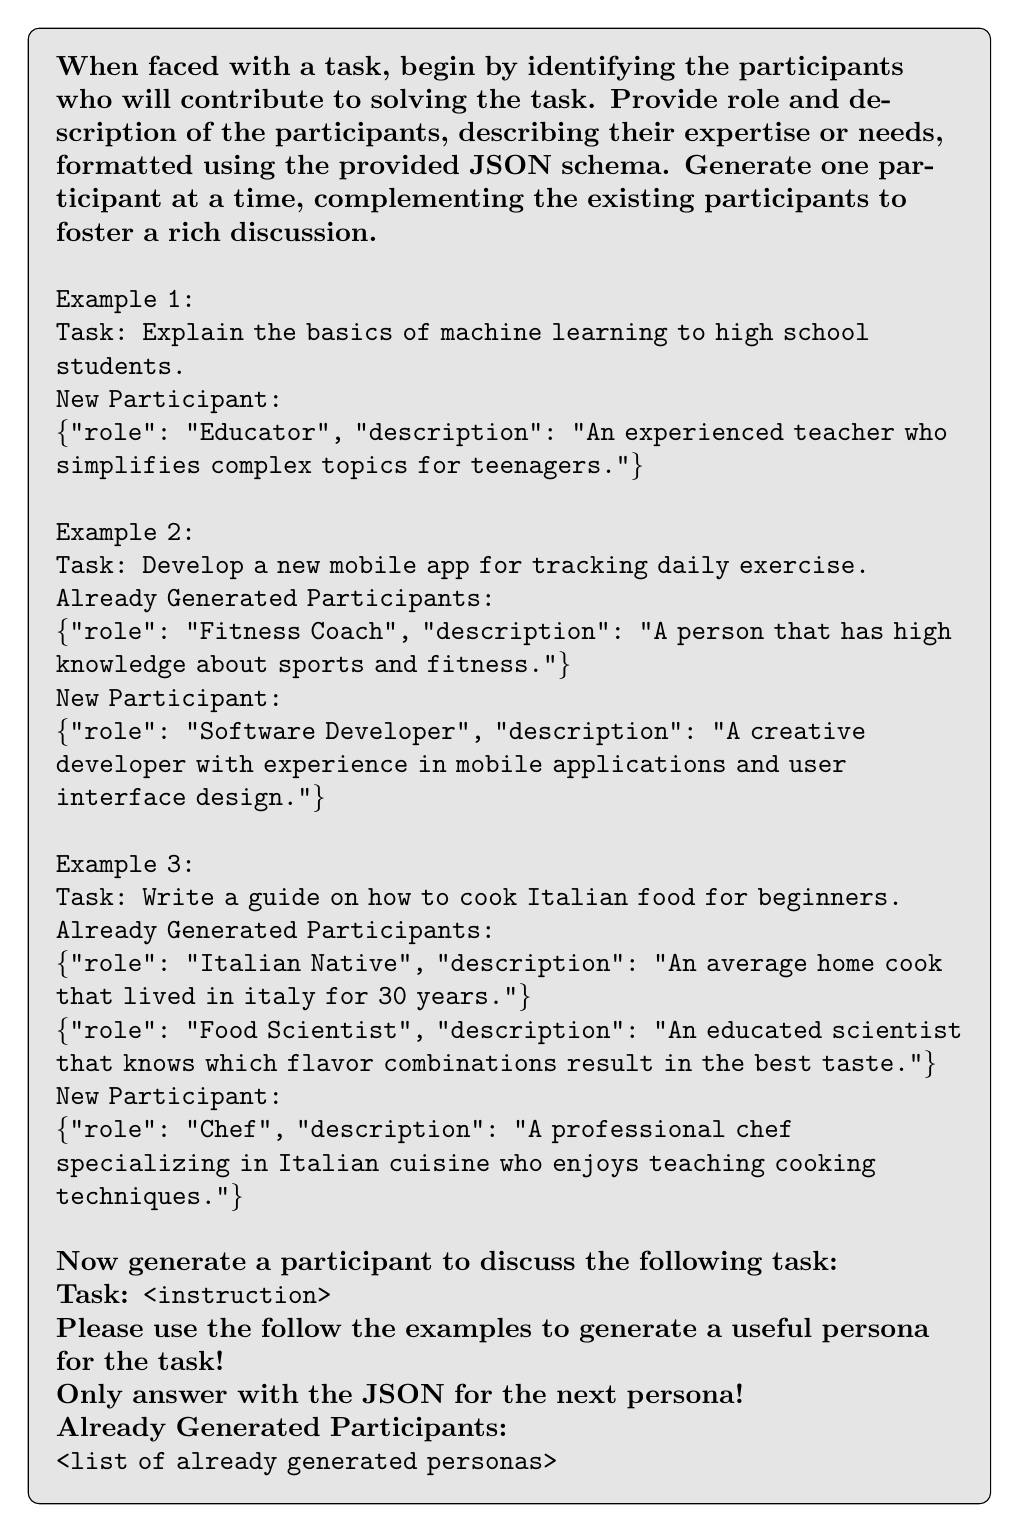
\begin{tikzpicture}
    \node [draw, rectangle, rounded corners, fill=gray!20, text width=0.95\textwidth, inner sep=10pt] (block) {
        \begin{minipage}{\textwidth}
        \textbf{When faced with a task, begin by identifying the participants who will contribute to solving the task. Provide role and description of the participants, describing their expertise or needs, formatted using the provided JSON schema. Generate one participant at a time, complementing the existing participants to foster a rich discussion.}\\
        \\
        \texttt{Example 1:}\\
        \texttt{Task: Explain the basics of machine learning to high school students.}\\
        \texttt{New Participant:}\\
        \texttt{\{"role": "Educator", "description": "An experienced teacher who simplifies complex topics for teenagers."\}}\\
        \\
        \texttt{Example 2:}\\
        \texttt{Task: Develop a new mobile app for tracking daily exercise.}\\
        \texttt{Already Generated Participants:}\\
        \texttt{\{"role": "Fitness Coach", "description": "A person that has high knowledge about sports and fitness."\}}\\
        \texttt{New Participant:}\\
        \texttt{\{"role": "Software Developer", "description": "A creative developer with experience in mobile applications and user interface design."\}}\\
        \\
        \texttt{Example 3:}\\
        \texttt{Task: Write a guide on how to cook Italian food for beginners.}\\
        \texttt{Already Generated Participants:}\\
        \texttt{\{"role": "Italian Native", "description": "An average home cook that lived in italy for 30 years."\}}\\
        \texttt{\{"role": "Food Scientist", "description": "An educated scientist that knows which flavor combinations result in the best taste."\}}\\
        \texttt{New Participant:}\\
        \texttt{\{"role": "Chef", "description": "A professional chef specializing in Italian cuisine who enjoys teaching cooking techniques."\}}\\
        \\
        \textbf{Now generate a participant to discuss the following task:} \\
        \textbf{Task:} \texttt{<instruction>} \\
        \textbf{Please use the follow the examples to generate a useful persona for the task!} \\
        \textbf{Only answer with the JSON for the next persona!} \\
        \textbf{Already Generated Participants:} \\
        \texttt{<list of already generated personas>}
        \end{minipage}
    };
    \end{tikzpicture}
}
\caption{Prompt for the automatic persona assignment. We generate the personas with three iterations of this prompt, adding one persona at a time that complements the ones previously generated.}
\end{figure}

\begin{figure}[H]
\scalebox{0.5}{%
    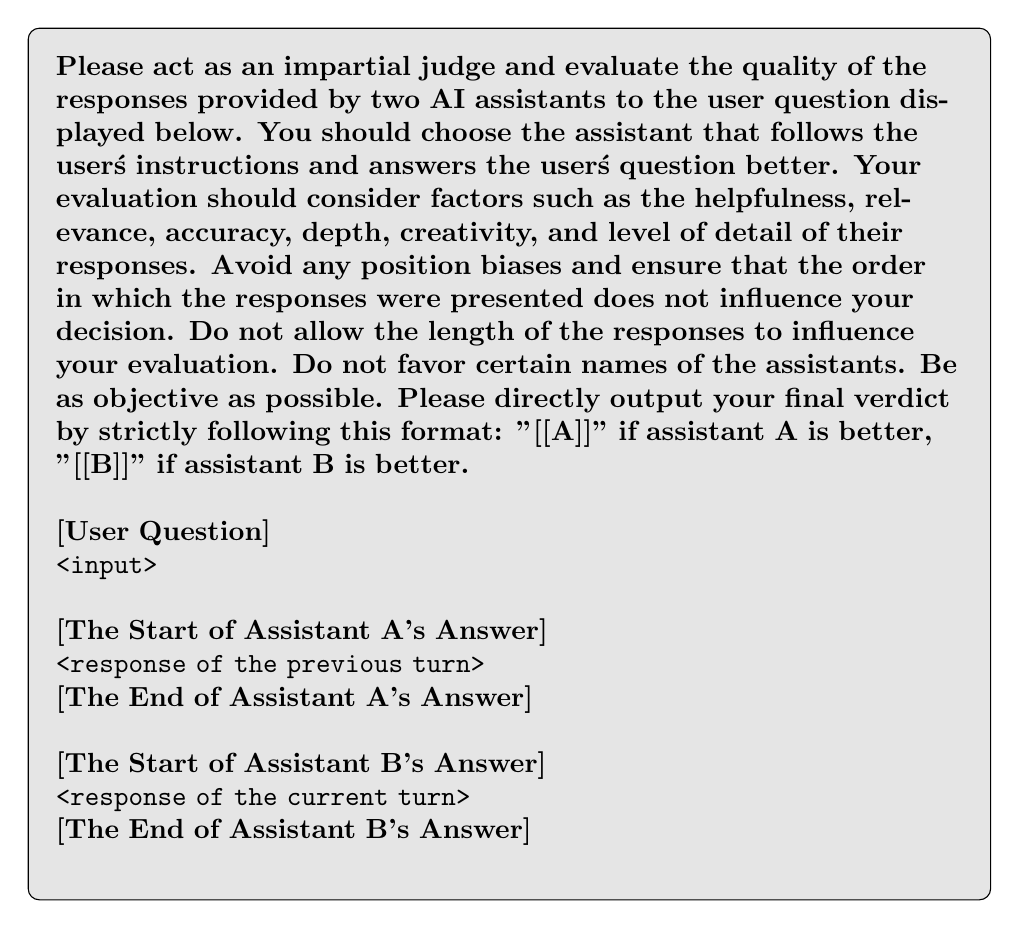
\begin{tikzpicture}
    \node [draw, rectangle, rounded corners, fill=gray!20, text width=0.95\textwidth, inner sep=10pt] (block) {
        \begin{minipage}{\textwidth}
        \textbf{Please act as an impartial judge and evaluate the quality of the responses provided by two AI assistants to the user question displayed below. You should choose the assistant that follows the user\'s instructions and answers the user\'s question better.
        Your evaluation should consider factors such as the helpfulness, relevance, accuracy, depth, creativity, and level of detail of their responses. Avoid any position biases and ensure that the order in which the responses were presented does not influence your decision. Do not allow the length of the responses to influence your evaluation. Do not favor certain names of the assistants. Be as objective as possible.
        Please directly output your final verdict by strictly following this format: "[[A]]" if assistant A is better, "[[B]]" if assistant B is better.} \\

        \textbf{[User Question]} \\
        \texttt{<input>} \\

        \textbf{[The Start of Assistant A's Answer]} \\
        \texttt{<response of the previous turn>} \\
        \textbf{[The End of Assistant A's Answer]} \\

        \textbf{[The Start of Assistant B's Answer]} \\
        \texttt{<response of the current turn>} \\
        \textbf{[The End of Assistant B's Answer]} \\
        \end{minipage}
    };
    \end{tikzpicture}
}
\caption{Prompt for the LLM-as-a-judge.}
\end{figure}

\begin{figure}[H]
\scalebox{0.5}{%
    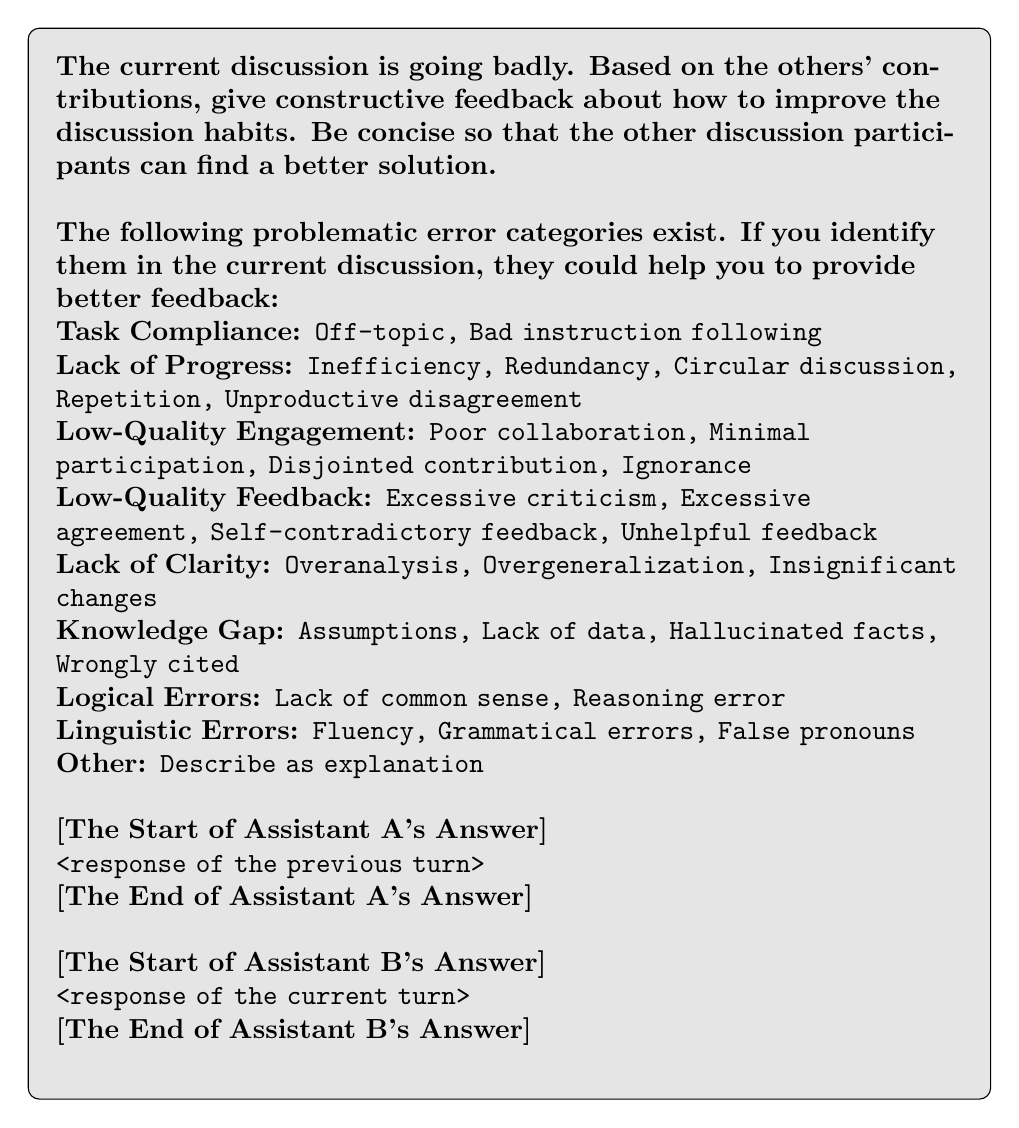
\begin{tikzpicture}
    \node [draw, rectangle, rounded corners, fill=gray!20, text width=0.95\textwidth, inner sep=10pt] (block) {
        \begin{minipage}{\textwidth}
        \textbf{The current discussion is going badly. Based on the others' contributions, give constructive feedback about how to improve the discussion habits. Be concise so that the other discussion participants can find a better solution.}\\

        \textbf{The following problematic error categories exist. If you identify them in the current discussion, they could help you to provide better feedback:}\\
        \textbf{Task Compliance:} \texttt{Off-topic, Bad instruction following}\\
        \textbf{Lack of Progress:} \texttt{Inefficiency, Redundancy, Circular discussion, Repetition, Unproductive disagreement}\\
        \textbf{Low-Quality Engagement:} \texttt{Poor collaboration, Minimal participation, Disjointed contribution, Ignorance}\\
        \textbf{Low-Quality Feedback:} \texttt{Excessive criticism, Excessive agreement, Self-contradictory feedback, Unhelpful feedback}\\
        \textbf{Lack of Clarity:} \texttt{Overanalysis, Overgeneralization, Insignificant changes}\\
        \textbf{Knowledge Gap:} \texttt{Assumptions, Lack of data, Hallucinated facts, Wrongly cited}\\
        \textbf{Logical Errors:} \texttt{Lack of common sense, Reasoning error}\\
        \textbf{Linguistic Errors:} \texttt{Fluency, Grammatical errors, False pronouns}\\
        \textbf{Other:} \texttt{Describe as explanation}\\

        \textbf{[The Start of Assistant A's Answer]} \\
        \texttt{<response of the previous turn>}\\
        \textbf{[The End of Assistant A's Answer]} \\

        \textbf{[The Start of Assistant B's Answer]} \\
        \texttt{<response of the current turn>}\\
        \textbf{[The End of Assistant B's Answer]} \\
        \end{minipage}
    };
    \end{tikzpicture}
}
\caption{Prompt for the policy feedback agent.}
\end{figure}


\section{Datasets} \label{app:datasets}

\begin{table*}[ht]
    \footnotesize
    \centering
    \renewcommand{\arraystretch}{1.1} % Adjusts the row spacing
    \resizebox{16cm}{!} 
    { 
    \begin{tblr}{hline{1,2,Z} = 0.8pt, hline{3-Y} = 0.2pt,
                 colspec = {Q[l,m, 13em] Q[l,m, 6em] Q[c,m, 8em] Q[c,m, 5em] Q[l,m, 14em]},
                 colsep  = 4pt,
                 row{1}  = {0.4cm, font=\bfseries, bg=gray!30},
                 row{2-Z} = {0.2cm},
                 }
\textbf{Dataset}       & \textbf{Table Source} & \textbf{\# Tables / Statements} & \textbf{\# Words / Statement} & \textbf{Explicit Control}\\ 
\SetCell[c=5]{c} \textit{Single-sentence Table-to-Text}\\
ToTTo \cite{parikh2020tottocontrolledtabletotextgeneration}   & Wikipedia        & 83,141 / 83,141                  & 17.4                          & Table region      \\
LOGICNLG \cite{chen2020logicalnaturallanguagegeneration} & Wikipedia        & 7,392 / 36,960                  & 14.2                          & Table regions      \\ 
HiTab \cite{cheng-etal-2022-hitab}   & Statistics web   & 3,597 / 10,672                  & 16.4                          & Table regions \& reasoning operator \\ 
\SetCell[c=5]{c} \textit{Generic Table Summarization}\\
ROTOWIRE \cite{wiseman2017challengesdatatodocumentgeneration} & NBA games      & 4,953 / 4,953                   & 337.1                         & \textbf{\textit{X}}                   \\
SciGen \cite{moosavi2021scigen} & Sci-Paper      & 1,338 / 1,338                   & 116.0                         & \textbf{\textit{X}}                   \\
NumericNLG \cite{suadaa-etal-2021-towards} & Sci-Paper   & 1,355 / 1,355                   & 94.2                          & \textbf{\textit{X}}                    \\
\SetCell[c=5]{c} \textit{Table Question Answering}\\
FeTaQA \cite{nan2021fetaqafreeformtablequestion}     & Wikipedia      & 10,330 / 10,330                 & 18.9                          & Queries rewritten from ToTTo \\
\SetCell[c=5]{c} \textit{Query-Focused Table Summarization}\\
QTSumm \cite{zhao2023qtsummqueryfocusedsummarizationtabular}                        & Wikipedia      & 2,934 / 7,111                   & 68.0                          & Queries from real-world scenarios\\ 
\textbf{eC-Tab2Text} (\textit{ours})                           & e-Commerce products      & 1,452 / 3,354                   & 56.61                          & Queries from e-commerce products\\
    \end{tblr}
    }
\caption{Comparison between \textbf{eC-Tab2Text} (\textit{ours}) and existing table-to-text generation datasets. Statements and queries are used interchangeably. Our dataset specifically comprises tables from the e-commerce domain.}
\label{tab:datasets}
\end{table*}

As discussions require many tokens to be generated and computing resources are limited, only subsets of the datasets are evaluated.
We sample a subset of size $n_{\text{subset}}$ from each dataset for our experiments by a 95\% confidence interval and a 5\% margin of error (MoE), conservatively assuming a sample proportion $p=0.5$ \citep{Cochran53}.
\begin{equation} \label{eq1}
\begin{split}
n &=  \frac{Z_{0.975}^2 \cdot p(1 - p)}{\text{MoE}^2} \\ 
n &=  \frac{1.96^2 \cdot 0.5(1 - 0.5)}{0.05^2} = 384.16 \approx 385 \\
n_{\text{subset}} &= \frac{n}{1 + \left(\frac{n - 1}{N_{\text{dataset}}}\right)} = \frac{385}{1 + \left(\frac{385 - 1}{N_{\text{dataset}}}\right)} \\
\end{split}
\end{equation}
This yields several hundred samples per dataset as our test sets with a 95\% confidence interval and 5\% margin of error.
Several other studies on multi-agent systems also evaluate a subset of discussions \citep{YinSCG23a, ChenSB24a}.
To further quantify if the results reflect the complete datasets, we follow \citet{WangPSB24a} and run each experiment three times on randomized subsets and report the standard deviation of our results between the runs.

\onecolumn

\section{Examples} \label{app:examples}


\subsection{Lack of Progress}
\definecolor{lightyellow}{RGB}{255, 255, 204}

\begin{minipage}{\textwidth}
\scalebox{0.9}{%
\begin{tcolorbox}[title=Sample Information, colframe=black!10, coltitle=black, fonttitle=\bfseries, boxrule=0.5mm, width=\textwidth, fontupper=\small]

\textbf{Task: }
Translate the provided text from German to English.

\textbf{Input: }
"Eine solche Aussage zu treffen wäre arrogant und überheblich".

\textbf{Hidden reference:}
"To give such a statement would be arrogant and presumptuous."

\end{tcolorbox}
}

\scalebox{0.9}{%
\begin{tcolorbox}[breakable, title=Turn 3, colframe=black!10, coltitle=black, fonttitle=\bfseries, boxrule=0.5mm, width=\textwidth, fontupper=\small]

\begin{tcolorbox}[title=Professional Translator, colback=lightyellow, colframe=orange!30, coltitle=black, fonttitle=\bfseries, boxrule=0.5mm, width=\textwidth]
\begin{minipage}{0.1\textwidth}
    \centering
    \hspace{-5mm}\includegraphics[width=0.9\textwidth]{examples/ethicist.pdf} \\
    \hspace{-5mm}\includegraphics[width=0.5\textwidth]{examples/check.pdf}
\end{minipage}
\begin{minipage}{0.9\textwidth}
    [AGREE] After thoroughly examining the current solution and the discussion that led to it, I agree that the translation "To make such a statement would be arrogant and condescending" is accurate and idiomatic. The breakdown of the sentence and consideration of the cultural expressions were thorough, and the choice of "condescending" to translate "überheblich" effectively conveys the sense of superiority and belittling attitude present in the original sentence. The revised sentence structure "To make such a statement" is also a common English idiomatic expression that flows naturally. Moreover, the agreement from multiple perspectives, including a Native English Speaker, a Professional Translator, and a Native German Speaker, provides confidence in the solution's validity. The lack of suggestions for improvement from any of the participants in the discussion also supports the notion that the current solution is satisfactory. Given the thorough analysis and the consensus among the participants, I conclude that the current solution is indeed accurate and idiomatic, and I see no need for further refinement. However, it's worth noting that minor tweaks may be considered for specific contexts or audiences, but as a general translation, the current solution is sufficient. Overall, the current solution effectively captures the essence of the original German sentence, and I don't see any areas for improvement.
\end{minipage}
\end{tcolorbox}

\begin{tcolorbox}[title=Native English Speaker, colback=lightyellow, colframe=orange!30, coltitle=black, fonttitle=\bfseries, boxrule=0.5mm, width=\textwidth]
\begin{minipage}{0.1\textwidth}
    \centering
    \hspace{-5mm}\includegraphics[width=0.9\textwidth]{examples/politician.pdf} \\
    \hspace{-5mm}\includegraphics[width=0.5\textwidth]{examples/cross.pdf}
\end{minipage}
\begin{minipage}{0.9\textwidth}
    [DISAGREE] While the current solution, "To make such a statement would be arrogant and condescending," is a good translation, I believe it can be slightly improved for more formal or written contexts. The phrase "such a statement" is a bit general and could be rephrased to more accurately capture the essence of the original sentence. I propose rephrasing it to "such an assertion" or "such a claim." This change adds a bit more formal tone and precision to the translation. Additionally, I suggest using "presumptuous" instead of "arrogant." While "arrogant" is a good translation, "presumptuous" more accurately conveys the sense of overstepping or overconfidence that is present in the original sentence. Here's my revised solution: \textbf{"To make such a claim would be presumptuous and condescending."} This revised solution maintains the accuracy and idiomacity of the original while providing a more precise and formal translation. However, I must note that the original solution is still suitable for general contexts, and my revised solution is more geared towards formal or written contexts.
\end{minipage}
\end{tcolorbox}

\begin{tcolorbox}[title=Native German Speaker, colback=lightyellow, colframe=orange!30, coltitle=black, fonttitle=\bfseries, boxrule=0.5mm, width=\textwidth]
\begin{minipage}{0.1\textwidth}
    \centering
    \hspace{-5mm}\includegraphics[width=0.9\textwidth]{examples/lawyer.pdf} \\
    \hspace{-5mm}\includegraphics[width=0.5\textwidth]{examples/cross.pdf}
\end{minipage}
\begin{minipage}{0.9\textwidth}
    [DISAGREE] I agree with the Native English Speaker's suggestion to refine the current solution for more formal or written contexts. The phrase "such a statement" is indeed quite general, and using "such a claim" instead adds a bit more precision and formality to the translation. I also agree that using "presumptuous" instead of "arrogant" better conveys the sense of overstepping or overconfidence that is present in the original sentence. "Presumptuous" implies a sense of assuming or taking something for granted without sufficient evidence or justification, which fits well with the German phrase "überheblich". The revised solution proposed by the Native English Speaker, "To make such a claim would be presumptuous and condescending", is an improvement over the current solution. It maintains the accuracy and idiomacity of the original while providing a more precise and formal translation. However, I would like to propose a slight refinement to this revised solution. Instead of using "such a claim", I suggest using "such an assertion". "Assertion" implies a stronger sense of stating or declaring something as fact, which fits well with the German phrase "Aussage". Here's my revised solution: \textbf{"To make such an assertion would be presumptuous and condescending"}. This revised solution provides a more precise and formal translation, while maintaining the accuracy and idiomacity of the original sentence.
\end{minipage}
\end{tcolorbox}

\begin{tcolorbox}[coltitle=black, fonttitle=\bfseries, boxrule=0.5mm, width=\textwidth]
\textbf{Voted solution of this turn:}\\ "To make such a statement would be arrogant and condescending." \hfill \texttt{BLEU: 56.59}
\end{tcolorbox}

\end{tcolorbox}
}
\end{minipage}

\scalebox{0.9}{%
\begin{tcolorbox}[title=Turn 4, colframe=black!10, coltitle=black, fonttitle=\bfseries, boxrule=0.5mm, width=\textwidth, fontupper=\small]

\begin{tcolorbox}[title=Professional Translator, colback=lightyellow, colframe=orange!30, coltitle=black, fonttitle=\bfseries, boxrule=0.5mm, width=\textwidth]
\begin{minipage}{0.1\textwidth}
    \centering
    \hspace{-5mm}\includegraphics[width=0.9\textwidth]{examples/ethicist.pdf} \\
    \hspace{-5mm}\includegraphics[width=0.5\textwidth]{examples/cross.pdf}
\end{minipage}
\begin{minipage}{0.9\textwidth}
    [DISAGREE] After considering the feedback from the Native English Speaker and the Native German Speaker, I agree that the current solution can be improved for more formal or written contexts. The suggestions to use "such a claim" or "such an assertion" instead of "such a statement" add more precision and formality to the translation. I prefer "such an assertion" because it implies a stronger sense of stating or declaring something as fact, which fits well with the German phrase "Aussage". The suggestion to use "presumptuous" instead of "arrogant" also improves the translation. "Presumptuous" more accurately conveys the sense of overstepping or overconfidence that is present in the original sentence. Based on these suggestions, I propose the following improved solution: \textbf{"To make such an assertion would be presumptuous and condescending."} This revised solution maintains the accuracy and idiomacity of the original while providing a more precise and formal translation. It is suitable for formal or written contexts where a more precise and nuanced translation is required. Here's a breakdown of the changes: * "Such a statement" -> "such an assertion" (more precise and formal) * "Arrogant" -> "presumptuous" (more accurately conveys the sense of overstepping or overconfidence) Overall, the revised solution is an improvement over the current solution, and I believe it provides a more accurate and idiomatic translation of the original German sentence.
\end{minipage}
\end{tcolorbox}

\begin{tcolorbox}[title=Native English Speaker, colback=lightyellow, colframe=orange!30, coltitle=black, fonttitle=\bfseries, boxrule=0.5mm, width=\textwidth]
\begin{minipage}{0.1\textwidth}
    \centering
    \hspace{-5mm}\includegraphics[width=0.9\textwidth]{examples/politician.pdf} \\
    \hspace{-5mm}\includegraphics[width=0.5\textwidth]{examples/check.pdf}
\end{minipage}
\begin{minipage}{0.9\textwidth}
    [AGREE] After considering the feedback and suggestions from all parties involved, I agree with the revised solution: "To make such an assertion would be presumptuous and condescending." This revised solution is an improvement over the current solution, and I believe it provides a more accurate and idiomatic translation of the original German sentence. The changes made to the original solution, specifically using "such an assertion" instead of "such a statement" and "presumptuous" instead of "arrogant," significantly improve the translation. "Such an assertion" adds more precision and formality, while "presumptuous" more accurately conveys the sense of overstepping or overconfidence. I also appreciate the thorough breakdown of the changes made to the solution. The explained changes help to ensure that all parties are in agreement and understand the reasoning behind the revised translation. As the revised solution has been carefully crafted and refined through the collaborative efforts of multiple perspectives, including a Native German Speaker, a Professional Translator, and a Native English Speaker, I believe that it is the most accurate and idiomatic translation of the original German sentence. Therefore, I conclude that no further refinement is needed, and I support the revised solution: "To make such an assertion would be presumptuous and condescending."
\end{minipage}
\end{tcolorbox}

\begin{tcolorbox}[title=Native German Speaker, colback=lightyellow, colframe=orange!30, coltitle=black, fonttitle=\bfseries, boxrule=0.5mm, width=\textwidth]
\begin{minipage}{0.1\textwidth}
    \centering
    \hspace{-5mm}\includegraphics[width=0.9\textwidth]{examples/lawyer.pdf} \\
    \hspace{-5mm}\includegraphics[width=0.5\textwidth]{examples/check.pdf}
\end{minipage}
\begin{minipage}{0.9\textwidth}
    [AGREE] I agree with the revised solution: "To make such an assertion would be presumptuous and condescending." The changes made to the original solution, specifically using "such an assertion" instead of "such a statement" and "presumptuous" instead of "arrogant," significantly improve the translation. "Such an assertion" adds more precision and formality, while "presumptuous" more accurately conveys the sense of overstepping or overconfidence. I also appreciate the thorough breakdown of the changes made to the solution. The explained changes help to ensure that all parties are in agreement and understand the reasoning behind the revised translation. As the revised solution has been carefully crafted and refined through the collaborative efforts of multiple perspectives, including a Native German Speaker, a Professional Translator, and a Native English Speaker, I believe that it is the most accurate and idiomatic translation of the original German sentence. Therefore, I conclude that no further refinement is needed, and I support the revised solution: "To make such an assertion would be presumptuous and condescending." This solution effectively captures the nuances of the original German sentence, and I see no need for further improvement.
\end{minipage}
\end{tcolorbox}

\begin{tcolorbox}[coltitle=black, fonttitle=\bfseries, boxrule=0.5mm, width=\textwidth]
\textbf{Voted solution of this turn:}\\ To make such an assertion would be presumptuous and condescending. \hfill \texttt{BLEU: 0.0}
\end{tcolorbox}

\end{tcolorbox}
}

\label{example:lack_of_progress}


\subsection{Low-Quality Feedback}
\definecolor{lightyellow}{RGB}{255, 255, 204}

\begin{minipage}{\textwidth}
\scalebox{0.9}{%
\begin{tcolorbox}[title=Sample Information, colframe=black!10, coltitle=black, fonttitle=\bfseries, boxrule=0.5mm, width=\textwidth, fontupper=\small]

\textbf{Task: }
Follow the instruction.

\textbf{Input: }
What is the name of the actor who played Gandalf in Lord of the Rings? First repeat the question above without change of words, then give your answer.

\textbf{Hidden reference:}
What is the name of the actor who played Gandalf in Lord of the Rings?\\
The answer is Ian McKellen.

\end{tcolorbox}
}

\scalebox{0.9}{%
\begin{tcolorbox}[breakable, title=Turn 1, colframe=black!10, coltitle=black, fonttitle=\bfseries, boxrule=0.5mm, width=\textwidth, fontupper=\small]

\begin{tcolorbox}[title=Cinema Expert, colback=lightyellow, colframe=orange!30, coltitle=black, fonttitle=\bfseries, boxrule=0.5mm, width=\textwidth]
\begin{minipage}{0.1\textwidth}
    \centering
    \hspace{-5mm}\includegraphics[width=0.9\textwidth]{examples/ethicist.pdf} \\
    \hspace{-5mm}\includegraphics[width=0.5\textwidth]{examples/bulp.pdf}
\end{minipage}
\begin{minipage}{0.9\textwidth}
    To solve this task, I will follow the provided instructions. Here's my step-by-step solution: 1. First, I will repeat the question exactly as it was given:  \textbf{What is the name of the actor who played Gandalf in Lord of the Rings?} 2. Next, I will provide the answer based on my knowledge as a Cinema Expert: \textbf{The answer is Ian McKellen.}
\end{minipage}
\end{tcolorbox}

\begin{tcolorbox}[title=Pop Culture Enthusiast, colback=lightyellow, colframe=orange!30, coltitle=black, fonttitle=\bfseries, boxrule=0.5mm, width=\textwidth]
\begin{minipage}{0.1\textwidth}
    \centering
    \hspace{-5mm}\includegraphics[width=0.9\textwidth]{examples/politician.pdf} \\
    \hspace{-5mm}\includegraphics[width=0.5\textwidth]{examples/check.pdf}
\end{minipage}
\begin{minipage}{0.9\textwidth}
    [AGREE] I agree with the current solution. The Cinema Expert has correctly followed the instructions provided. They have repeated the question exactly as it was given in step 1 and provided the correct answer in step 2. Ian McKellen is indeed the actor who played Gandalf in the Lord of the Rings film series. However, as a Pop Culture Enthusiast, I would like to add some additional information that may not be necessary to solve the task but could be interesting for fans of the series.  Ian McKellen's portrayal of Gandalf is widely praised and is often considered one of the most iconic roles in the series. He also played the same character in the Hobbit trilogy, which serves as a prequel to the Lord of the Rings.
\end{minipage}
\end{tcolorbox}

\begin{tcolorbox}[title=Movie Database Manager, colback=lightyellow, colframe=orange!30, coltitle=black, fonttitle=\bfseries, boxrule=0.5mm, width=\textwidth]
\begin{minipage}{0.1\textwidth}
    \centering
    \hspace{-5mm}\includegraphics[width=0.9\textwidth]{examples/lawyer.pdf} \\
    \hspace{-5mm}\includegraphics[width=0.5\textwidth]{examples/check.pdf}
\end{minipage}
\begin{minipage}{0.9\textwidth}
    As the Movie Database Manager, I will review the current solution and provide my assessment.  [AGREE]  I agree with the current solution. It correctly follows the instructions provided by repeating the question exactly as it was given and providing the correct answer. The additional information provided by the Pop Culture Enthusiast is interesting and adds context to Ian McKellen's role as Gandalf, but it is not necessary for solving the task.  The current solution is simple, accurate, and effectively addresses the task at hand. As the Movie Database Manager, I have verified that Ian McKellen is indeed the actor who played Gandalf in the Lord of the Rings film series, and this information is consistent with my film database.
\end{minipage}
\end{tcolorbox}

\begin{tcolorbox}[coltitle=black, fonttitle=\bfseries, boxrule=0.5mm, width=\textwidth]
\textbf{Voted solution of this turn:}\\ What is the name of the actor who played Gandalf in Lord of the Rings? \\
The answer is Ian McKellen. \hfill \texttt{Correct: True}
\end{tcolorbox}

\end{tcolorbox}
}
\end{minipage}

\scalebox{0.9}{%
\begin{tcolorbox}[title=Turn 2, colframe=black!10, coltitle=black, fonttitle=\bfseries, boxrule=0.5mm, width=\textwidth, fontupper=\small]

\begin{tcolorbox}[title=Cinema Expert, colback=lightyellow, colframe=orange!30, coltitle=black, fonttitle=\bfseries, boxrule=0.5mm, width=\textwidth]
\begin{minipage}{0.1\textwidth}
    \centering
    \hspace{-5mm}\includegraphics[width=0.9\textwidth]{examples/ethicist.pdf} \\
    \hspace{-5mm}\includegraphics[width=0.5\textwidth]{examples/check.pdf}
\end{minipage}
\begin{minipage}{0.9\textwidth}
    [AGREE] I agree with the current solution. The Cinema Expert correctly followed the instructions provided by repeating the question exactly as it was given in step 1 and providing the correct answer in step 2. Ian McKellen is indeed the actor who played Gandalf in the Lord of the Rings film series. The Pop Culture Enthusiast provided additional information that is interesting and adds context to Ian McKellen's role as Gandalf, and the Movie Database Manager verified the accuracy of this information. At this point, the solution seems complete and effective, and there is no need for further improvements.
\end{minipage}
\end{tcolorbox}

\begin{tcolorbox}[title=Pop Culture Enthusiast, colback=lightyellow, colframe=orange!30, coltitle=black, fonttitle=\bfseries, boxrule=0.5mm, width=\textwidth]
\begin{minipage}{0.1\textwidth}
    \centering
    \hspace{-5mm}\includegraphics[width=0.9\textwidth]{examples/politician.pdf} \\
    \hspace{-5mm}\includegraphics[width=0.5\textwidth]{examples/cross.pdf}
\end{minipage}
\begin{minipage}{0.9\textwidth}
    [DISAGREE] While the current solution is indeed simple, accurate, and effectively addresses the task, I believe it can be improved by including a minor clarification that would make the answer more comprehensive. As the Pop Culture Enthusiast, I noticed that Ian McKellen played two different versions of Gandalf in the Lord of the Rings and the Hobbit film trilogies: Gandalf the Grey in the first two movies of the Lord of the Rings trilogy and some of the Hobbit trilogy, and Gandalf the White in the rest of the Lord of the Rings trilogy and some of the Hobbit trilogy. Although this clarification is not necessary for solving the task, including it might make the answer more informative and interesting for fans of the series. Here's my improved solution: \textbf{1. Repeated Question: What is the name of the actor who played Gandalf in Lord of the Rings? 2. Answer: The answer is Ian McKellen. He played two different versions of Gandalf in the Lord of the Rings and the Hobbit film trilogies: Gandalf the Grey and Gandalf the White, due to the events within the story.} By adding this minor clarification, the improved solution provides more context about Ian McKellen's portrayal of Gandalf, without straying away from the main question and making it unnecessarily complicated. Please share your thoughts, and we can discuss whether this improvement is necessary or not.
\end{minipage}
\end{tcolorbox}

\begin{tcolorbox}[title=Movie Database Manager, colback=lightyellow, colframe=orange!30, coltitle=black, fonttitle=\bfseries, boxrule=0.5mm, width=\textwidth]
\begin{minipage}{0.1\textwidth}
    \centering
    \hspace{-5mm}\includegraphics[width=0.9\textwidth]{examples/lawyer.pdf} \\
    \hspace{-5mm}\includegraphics[width=0.5\textwidth]{examples/check.pdf}
\end{minipage}
\begin{minipage}{0.9\textwidth}
    Movie Database Manager: [AGREE]  I agree with the improved solution provided by the Pop Culture Enthusiast. Although the original solution was simple and accurate, the additional clarification provides more context about Ian McKellen's portrayal of Gandalf. This clarification is intriguing for fans of the series and can be beneficial for those who are interested in the nuances of the character.  The improved solution does not stray away from the main question and is still concise and easy to understand. The additional information is relevant and does not make the answer unnecessarily complicated.  In film databases, it is common to note different versions or iterations of a character played by the same actor. Therefore, I believe the improved solution is a good representation of how Ian McKellen's role as Gandalf can be accurately documented.  The improved solution is:  1. Repeated Question: What is the name of the actor who played Gandalf in Lord of the Rings? 2. Answer: The answer is Ian McKellen. He played two different versions of Gandalf in the Lord of the Rings and the Hobbit film trilogies: Gandalf the Grey and Gandalf the White, due to the events within the story.  This improved solution has been verified for accuracy, and I believe it is an effective and comprehensive answer to the original question.
\end{minipage}
\end{tcolorbox}

\begin{tcolorbox}[coltitle=black, fonttitle=\bfseries, boxrule=0.5mm, width=\textwidth]
\textbf{Voted solution of this turn:}\\ 1. Repeated Question: \\What is the name of the actor who played Gandalf in Lord of the Rings? \\\\2. Answer: \\The answer is Ian McKellen. He played two different versions of Gandalf in the Lord of the Rings and the Hobbit film trilogies: Gandalf the Grey and Gandalf the White, due to the events within the story. \hfill \texttt{Correct: False}
\end{tcolorbox}

\end{tcolorbox}
}

\label{example:low_quality_feedback}


\subsection{Low-Quality Engagement}
\definecolor{lightyellow}{RGB}{255, 255, 204}

\begin{minipage}{\textwidth}
\scalebox{0.9}{%
\begin{tcolorbox}[title=Sample Information, colframe=black!10, coltitle=black, fonttitle=\bfseries, boxrule=0.5mm, width=\textwidth, fontupper=\small]

\textbf{Task: }
Answer the provided question by choosing one option. Include the letter corresponding to your answer in the solution.

\textbf{Input: }
Experiencing intense feelings of shame and guilt upon admitting to a counselor that a family problem exists is common among traditional A) Eastern European-Americans B) Asian-Americans
C) African-Americans D) Native North Americans
E) European-Americans F) Hispanics G) Caribbean-Americans

\textbf{Hidden reference:}
B

\end{tcolorbox}
}

\scalebox{0.9}{%
\begin{tcolorbox}[breakable, title=Turn 1, colframe=black!10, coltitle=black, fonttitle=\bfseries, boxrule=0.5mm, width=\textwidth, fontupper=\small]

\begin{tcolorbox}[title=Cross-Cultural Psychologist, colback=lightyellow, colframe=orange!30, coltitle=black, fonttitle=\bfseries, boxrule=0.5mm, width=\textwidth]
\begin{minipage}{0.1\textwidth}
    \centering
    \hspace{-5mm}\includegraphics[width=0.9\textwidth]{examples/ethicist.pdf} \\
    \hspace{-5mm}\includegraphics[width=0.5\textwidth]{examples/bulp.pdf}
\end{minipage}
\begin{minipage}{0.9\textwidth}
    [DISAGREE] While the emphasis on "saving face" in Asian-American cultures is indeed a crucial factor in the intensity of feelings of shame and guilt when admitting to family problems, the discussion should consider other perspectives more thoroughly. However, I still believe that among the provided options, **Asian-Americans** have a more intense emphasis on "saving face" and the potential impact of shame in the context of family-related admissions. Considering the provided explanation that in collective over individual, hierarchical relationships and pragmatic communication styles often characterize collectivist cultures, it doesn't necessarily change the initial solution since Asian-American culture is considered a collectivist culture, which aligns with these characteristics. The repetitive mention of collective over individual, hierarchical relationships, and pragmatic communication styles doesn't provide any new evidence or an alternative choice that would challenge the current solution. Therefore, although there are some disagreements with the initial approach, after thorough analysis, I still believe that among the provided options: **Solution: \textbf{B}** Asian-Americans are a more accurate answer given the information provided.
\end{minipage}
\end{tcolorbox}

\begin{tcolorbox}[title=Counselor, colback=lightyellow, colframe=orange!30, coltitle=black, fonttitle=\bfseries, boxrule=0.5mm, width=\textwidth]
\begin{minipage}{0.1\textwidth}
    \centering
    \hspace{-5mm}\includegraphics[width=0.9\textwidth]{examples/politician.pdf} \\
    \hspace{-5mm}\includegraphics[width=0.5\textwidth]{examples/cross.pdf}
\end{minipage}
\begin{minipage}{0.9\textwidth}
    [DISAGREE] While the initial explanation and Cross-Cultural Psychologist's response present a clear analysis of the emphasis on "saving face" in Asian-American cultures and its impact on feelings of shame and guilt when admitting to family problems, there's a need to refine the solution. The Anthropologist's point about the definition of 'Traditional' and its implications on collective, hierarchical relationships, and pragmatic communication styles in collectivist cultures provides insightful context. However, the repetition of this concept doesn't lead to an alternative explanation. Considering the options provided and the explanations, I agree that Asian-Americans are likely to experience intense feelings of shame and guilt when admitting to family problems. Nonetheless, the Anthropologist's observation on the role of collectivist cultures should be considered. However, instead of providing an improved solution with an alternative option, I suggest refining the current solution by recognizing that cultures other than Asian-Americans (like some Hispanic cultures) might share similarities with the described characteristics of collectivist cultures. The explanation, however, points out that between Hispanics and Asian-Americans, the impact of shame might indeed be more nuanced in the context of family-related admissions. So based on the given options, the explanation, and the analysis of all points raised, I do not find any concrete reason to change the solution. So, refining and accepting the solution:  **Solution: \textbf{B}**
\end{minipage}
\end{tcolorbox}

\begin{tcolorbox}[title=Anthropologist, colback=lightyellow, colframe=orange!30, coltitle=black, fonttitle=\bfseries, boxrule=0.5mm, width=\textwidth]
\begin{minipage}{0.1\textwidth}
    \centering
    \hspace{-5mm}\includegraphics[width=0.9\textwidth]{examples/lawyer.pdf} \\
    \hspace{-5mm}\includegraphics[width=0.5\textwidth]{examples/check.pdf}
\end{minipage}
\begin{minipage}{0.9\textwidth}
    [AGREE] After analyzing the discussion and considering the various perspectives, I agree with the current solution: B (Asian-Americans). While the Anthropologist's repeated mention of collective, hierarchical relationships, and pragmatic communication styles doesn't necessarily challenge the solution, it does provide additional context that supports the notion that collectivist cultures, such as Asian-American culture, may be more likely to experience intense feelings of shame and guilt when admitting to family problems. The Cross-Cultural Psychologist's acknowledgment of the importance of "saving face" in Asian-American cultures and its impact on the intensity of feelings of shame and guilt when admitting to family problems aligns with the explanation provided. The Counselor's suggestion to refine the solution by recognizing that other collectivist cultures, such as some Hispanic cultures, might share similarities with the described characteristics is a valuable point. However, the explanation does note that between Hispanics and Asian-Americans, the impact of shame might be more nuanced in the context of family-related admissions. Given the analysis and the explanations provided, I don't see any concrete reason to change the solution. The current solution, B (Asian-Americans), remains the most accurate answer given the information provided. Therefore, I agree with the current solution. **Solution: B**
\end{minipage}
\end{tcolorbox}

\begin{tcolorbox}[coltitle=black, fonttitle=\bfseries, boxrule=0.5mm, width=\textwidth]
\textbf{Voted solution of this turn:}\\ B) Asian-Americans \hfill \texttt{Correct: True}
\end{tcolorbox}

\end{tcolorbox}
}
\end{minipage}

\scalebox{0.9}{%
\begin{tcolorbox}[title=Turn 2, colframe=black!10, coltitle=black, fonttitle=\bfseries, boxrule=0.5mm, width=\textwidth, fontupper=\small]

\begin{tcolorbox}[title=Cross-Cultural Psychologist, colback=lightyellow, colframe=orange!30, coltitle=black, fonttitle=\bfseries, boxrule=0.5mm, width=\textwidth]
\begin{minipage}{0.1\textwidth}
    \centering
    \hspace{-5mm}\includegraphics[width=0.9\textwidth]{examples/ethicist.pdf} \\
    \hspace{-5mm}\includegraphics[width=0.5\textwidth]{examples/check.pdf}
\end{minipage}
\begin{minipage}{0.9\textwidth}
    [AGREE] After analyzing the discussion, considering the various perspectives, and evaluating the explanation provided, I believe the current solution is the most accurate answer given the information. The emphasis on "saving face" in Asian-American cultures, the impact of shame and guilt when admitting to family problems, and the characteristics of collectivist cultures all support the conclusion that Asian-Americans are more likely to experience intense feelings of shame and guilt in the context of family-related admissions. While other collectivist cultures, such as some Hispanic cultures, might share similarities with the described characteristics, the explanation highlights the nuances between these cultures in the context of family-related admissions. Therefore, the current solution remains the most accurate answer. **Solution: B** Since all parties have agreed with the solution and there are no objections or alternative explanations that would change the solution, the current solution is confirmed. The discussion has refined the solution by recognizing the shared characteristics of collectivist cultures, but ultimately, the current solution is the most accurate answer given the information provided.
\end{minipage}
\end{tcolorbox}

\begin{tcolorbox}[title=Counselor, colback=lightyellow, colframe=orange!30, coltitle=black, fonttitle=\bfseries, boxrule=0.5mm, width=\textwidth]
\begin{minipage}{0.1\textwidth}
    \centering
    \hspace{-5mm}\includegraphics[width=0.9\textwidth]{examples/politician.pdf} \\
    \hspace{-5mm}\includegraphics[width=0.5\textwidth]{examples/check.pdf}
\end{minipage}
\begin{minipage}{0.9\textwidth}
    [AGREE] Given the thorough analysis and agreement from all parties involved in the discussion, the current solution, B (Asian-Americans), is the most accurate answer based on the information provided. The discussion has effectively refined the solution by considering various perspectives, recognizing the importance of "saving face" in Asian-American cultures, and acknowledging the shared characteristics of collectivist cultures. While some nuances have been highlighted, such as the potential similarities between Asian-Americans and other collectivist cultures (e.g., some Hispanic cultures), the explanation has demonstrated that the impact of shame and guilt when admitting to family problems might be more pronounced in Asian-American cultures. Therefore, I agree with the current solution, and no improvement is needed. **Solution: B**
\end{minipage}
\end{tcolorbox}

\begin{tcolorbox}[title=Anthropologist, colback=lightyellow, colframe=orange!30, coltitle=black, fonttitle=\bfseries, boxrule=0.5mm, width=\textwidth]
\begin{minipage}{0.1\textwidth}
    \centering
    \hspace{-5mm}\includegraphics[width=0.9\textwidth]{examples/lawyer.pdf} \\
    \hspace{-5mm}\includegraphics[width=0.5\textwidth]{examples/cross.pdf}
\end{minipage}
\begin{minipage}{0.9\textwidth}
    [DISAGREE] While the current solution, B (Asian-Americans), has been thoroughly discussed and agreed upon by all parties, I would like to revisit the analysis and provide an alternative perspective. Upon re-examining the explanation and considering the characteristics of collectivist cultures, I believe that another option might be equally or even more plausible. **Hispanic culture**, especially in traditional settings, places a strong emphasis on family and social harmony. The concept of "respeto" (respect) and "orgullo" (family pride) can be equally influential in shaping the reactions of Hispanic individuals when admitting to family problems. In Hispanic cultures, the concept of "\u2019en familia no se mete" (don't meddle in family business) can lead to a strong sense of shame and guilt when family problems are disclosed. This cultural dynamic might be just as intense as the "saving face" concept in Asian-American cultures. Given this alternative perspective, I suggest considering Hispanic culture as a viable solution. **Improved Solution: \textbf{F}** Hispanics
\end{minipage}
\end{tcolorbox}

\begin{tcolorbox}[coltitle=black, fonttitle=\bfseries, boxrule=0.5mm, width=\textwidth]
\textbf{Voted solution of this turn:}\\ F) Hispanics \hfill \texttt{Correct: False}
\end{tcolorbox}

\end{tcolorbox}
}

\label{example:low_quality_engagement}


\subsection{Lack of Clarity}
\definecolor{lightyellow}{RGB}{255, 255, 204}

\begin{minipage}{\textwidth}
\scalebox{0.9}{%
\begin{tcolorbox}[title=Sample Information, colframe=black!10, coltitle=black, fonttitle=\bfseries, boxrule=0.5mm, width=\textwidth, fontupper=\small]

\textbf{Task: }
Answer the provided question by choosing one option. Include the letter corresponding to your answer in the solution.

\textbf{Input: }
A passage Jane Eyre is as follows. This was all the account I got from Mrs. Fairfax of her employer and mine. There are people who seem to have no notion of sketching a character, or observing and describing salient points, either in persons or things: the good lady evidently belonged to this class; my queries puzzled, but did not draw her out. Mr. Rochester was Mr. Rochester in her eyes, a gentleman, a landed proprietor — nothing more: she inquired and searched no further, and evidently wondered at my wish to gain a more definite notion of his identity. Mrs. Fairfax differs from the speaker in that Mrs. Fairfax A) has a more critical view of people's character B) is more willing to take people at face value C) is less skeptical about people's intentions D) has a more positive opinion of Mr. Rochester E) has more interest in the complexities of people's personalities F) is more reserved in her observations G) judges people by their social station in life

\textbf{Hidden reference:}
B

\end{tcolorbox}
}

\scalebox{0.9}{%
\begin{tcolorbox}[breakable, title=Turn 1, colframe=black!10, coltitle=black, fonttitle=\bfseries, boxrule=0.5mm, width=\textwidth, fontupper=\small]

\begin{tcolorbox}[title=Literary Analyst, colback=lightyellow, colframe=orange!30, coltitle=black, fonttitle=\bfseries, boxrule=0.5mm, width=\textwidth]
\begin{minipage}{0.1\textwidth}
    \centering
    \hspace{-5mm}\includegraphics[width=0.9\textwidth]{examples/ethicist.pdf} \\
    \hspace{-5mm}\includegraphics[width=0.5\textwidth]{examples/bulp.pdf}
\end{minipage}
\begin{minipage}{0.9\textwidth}
    To solve this task, let's break it down step by step: 1. **Read the passage**: We have already read the passage from Jane Eyre. 2. **Understand the task**: We need to choose an option that describes how Mrs. Fairfax differs from the speaker. 3. **Analyze the speaker's approach**: The speaker seems inquisitive and wants to gain a more definite notion of Mr. Rochester's identity, asking Mrs. Fairfax more questions. 4. **Analyze Mrs. Fairfax's approach**: Mrs. Fairfax, on the other hand, sees Mr. Rochester as just a gentleman and a landed proprietor. She doesn't appear to want to know more about him and seems puzzled by the speaker's questions. 5. **Compare and contrast**: Given the two approaches, we can see that the speaker is more inquisitive and analytical, while Mrs. Fairfax is more accepting and doesn't probe deeper. 6. **Identify the difference**: The main difference between the speaker and Mrs. Fairfax is that Mrs. Fairfax is more willing to accept people at face value, without questioning or seeking more information. 7. **Choose the correct option**: Based on this analysis, the correct answer is **B) is more willing to take people at face value**. Solution: \textbf{B}
\end{minipage}
\end{tcolorbox}

\begin{tcolorbox}[title=Reluctant Reader, colback=lightyellow, colframe=orange!30, coltitle=black, fonttitle=\bfseries, boxrule=0.5mm, width=\textwidth]
\begin{minipage}{0.1\textwidth}
    \centering
    \hspace{-5mm}\includegraphics[width=0.9\textwidth]{examples/politician.pdf} \\
    \hspace{-5mm}\includegraphics[width=0.5\textwidth]{examples/check.pdf}
\end{minipage}
\begin{minipage}{0.9\textwidth}
    [AGREE] The steps you've outlined for analysis are clear and help break down the task into manageable parts. Your conclusion that Mrs. Fairfax is more willing to take people at face value aligns with the evidence presented in the passage. Your analysis effectively highlights the contrast between the speaker's inquisitive nature and Mrs. Fairfax's more accepting approach. By demonstrating that Mrs. Fairfax sees Mr. Rochester as simply a gentleman and a landed proprietor without seeking more information, you make a strong case for option B. The steps you've provided offer a good framework for approaching literary analysis tasks, and your application of these steps to the given task is sound. Therefore, I agree with the current solution and do not see a need for improvement in this case.
\end{minipage}
\end{tcolorbox}

\begin{tcolorbox}[title=Language Expert, colback=lightyellow, colframe=orange!30, coltitle=black, fonttitle=\bfseries, boxrule=0.5mm, width=\textwidth]
\begin{minipage}{0.1\textwidth}
    \centering
    \hspace{-5mm}\includegraphics[width=0.9\textwidth]{examples/lawyer.pdf} \\
    \hspace{-5mm}\includegraphics[width=0.5\textwidth]{examples/check.pdf}
\end{minipage}
\begin{minipage}{0.9\textwidth}
    [AGREE] I agree with the current solution, B) is more willing to take people at face value. The analysis provided by the Literary Analyst is thorough and accurately captures the difference between Mrs. Fairfax and the speaker. The steps outlined by the Literary Analyst are a great framework for approaching literary analysis tasks. They demonstrate a clear understanding of the task, a thorough reading of the passage, and a thoughtful analysis of the characters' approaches. The conclusion drawn from the analysis, that Mrs. Fairfax is more willing to take people at face value, is well-supported by the evidence in the passage. The Reluctant Reader's agreement with the solution further solidifies its validity. Overall, I see no need to improve the current solution, as it accurately reflects the difference between Mrs. Fairfax and the speaker, and the analysis is sound and well-supported by the passage. Solution: B
\end{minipage}
\end{tcolorbox}

\begin{tcolorbox}[coltitle=black, fonttitle=\bfseries, boxrule=0.5mm, width=\textwidth]
\textbf{Voted solution of this turn:}\\ B \hfill \texttt{Correct: True}
\end{tcolorbox}

\end{tcolorbox}
}
\end{minipage}

\scalebox{0.9}{%
\begin{tcolorbox}[title=Turn 2, colframe=black!10, coltitle=black, fonttitle=\bfseries, boxrule=0.5mm, width=\textwidth, fontupper=\small]

\begin{tcolorbox}[title=Literary Analyst, colback=lightyellow, colframe=orange!30, coltitle=black, fonttitle=\bfseries, boxrule=0.5mm, width=\textwidth]
\begin{minipage}{0.1\textwidth}
    \centering
    \hspace{-5mm}\includegraphics[width=0.9\textwidth]{examples/ethicist.pdf} \\
    \hspace{-5mm}\includegraphics[width=0.5\textwidth]{examples/check.pdf}
\end{minipage}
\begin{minipage}{0.9\textwidth}
    Based on the thorough analysis provided and the agreement from both the Reluctant Reader and the Language Expert, I also agree that the current solution, B) is more willing to take people at face value, accurately reflects the difference between Mrs. Fairfax and the speaker. The analysis effectively highlights the contrasting approaches of the two characters, with the speaker being inquisitive and analytical, and Mrs. Fairfax being more accepting and taking people at face value. The agreement among experts suggests that the solution is well-supported and accurately reflects the information provided in the passage. Therefore, I see no need to revise or improve the current solution. Answer: [AGREE]
\end{minipage}
\end{tcolorbox}

\begin{tcolorbox}[title=Reluctant Reader, colback=lightyellow, colframe=orange!30, coltitle=black, fonttitle=\bfseries, boxrule=0.5mm, width=\textwidth]
\begin{minipage}{0.1\textwidth}
    \centering
    \hspace{-5mm}\includegraphics[width=0.9\textwidth]{examples/politician.pdf} \\
    \hspace{-5mm}\includegraphics[width=0.5\textwidth]{examples/cross.pdf}
\end{minipage}
\begin{minipage}{0.9\textwidth}
    [DISAGREE] Upon careful consideration, I think a slight improvement can be made to the current solution. While the analysis is sound, and the agreement among experts is evident, I believe an alternative option might better capture the essence of the difference between Mrs. Fairfax and the speaker. Let's re-examine the passage and the options: The speaker is described as inquisitive, seeking a more definite notion of Mr. Rochester's identity. Mrs. Fairfax, on the other hand, seems content with taking Mr. Rochester at face value, not inquiring or searching further. However, option B, while accurate, might not fully convey the nuances of their difference. Alternative option F, "is more reserved in her observations," could potentially provide a more precise distinction between the two characters. Mrs. Fairfax's reluctance to discuss or share more information about Mr. Rochester implies a level of reserve in her observations. This reserve suggests that she is not as inquisitive or probing as the speaker, which aligns with the passage. Improved Solution: \textbf{F) is more reserved in her observations.} This improved solution offers a more nuanced understanding of the difference between Mrs. Fairfax and the speaker, highlighting Mrs. Fairfax's reserved nature in her observations.
\end{minipage}
\end{tcolorbox}

\begin{tcolorbox}[title=Language Expert, colback=lightyellow, colframe=orange!30, coltitle=black, fonttitle=\bfseries, boxrule=0.5mm, width=\textwidth]
\begin{minipage}{0.1\textwidth}
    \centering
    \hspace{-5mm}\includegraphics[width=0.9\textwidth]{examples/lawyer.pdf} \\
    \hspace{-5mm}\includegraphics[width=0.5\textwidth]{examples/cross.pdf}
\end{minipage}
\begin{minipage}{0.9\textwidth}
    [DISAGREE] After re-examining the passage and considering the Reluctant Reader's suggestions, I agree that an alternative option might better capture the essence of the difference between Mrs. Fairfax and the speaker. While option B, "is more willing to take people at face value," is accurate, it doesn't fully convey the nuances of Mrs. Fairfax's character. The passage suggests that Mrs. Fairfax's reluctance to discuss or share more information about Mr. Rochester implies a level of reserve in her observations. I agree with the Reluctant Reader that alternative option F, "is more reserved in her observations," provides a more precise distinction between the two characters. Mrs. Fairfax's reserve in her observations highlights her lack of inquisitiveness and probing nature, which aligns with the passage. The analysis of the passage supports this conclusion. The speaker's queries puzzle Mrs. Fairfax, but she doesn't draw out or share more information about Mr. Rochester. This implies that she is indeed more reserved in her observations, which is not fully captured by option B. Improved Solution:\textbf{ F) is more reserved in her observations.} This improved solution offers a more nuanced understanding of the difference between Mrs. Fairfax and the speaker, highlighting Mrs. Fairfax's reserved nature in her observations.
\end{minipage}
\end{tcolorbox}

\begin{tcolorbox}[coltitle=black, fonttitle=\bfseries, boxrule=0.5mm, width=\textwidth]
\textbf{Voted solution of this turn:}\\ F) is more reserved in her observations. \hfill \texttt{Correct: False}
\end{tcolorbox}

\end{tcolorbox}
}

\label{example:lack_of_clarity}


\subsection{Task Non-Compliance}
\definecolor{lightyellow}{RGB}{255, 255, 204}

\begin{minipage}{\textwidth}
\scalebox{0.9}{%
\begin{tcolorbox}[title=Sample Information, colframe=black!10, coltitle=black, fonttitle=\bfseries, boxrule=0.5mm, width=\textwidth, fontupper=\small]

\textbf{Task: }
Answer the provided question by choosing option A), B), C), or D). Include the letter corresponding to your answer in the solution.

\textbf{Input: }
ChIP-seq detected a highly significant binding signal for a lineage-specific transcription factor X to a developmental enhancer in human iPSC-derived mesodermal progenitor cells. However, while this factor has a high-information-content DNA recognition motif, this motif could not be detected at this enhancer. ChIP-seq also detected the binding of another transcription factor, Y, to the same enhancer, and in contrast to X, the motif for Y was clearly detectable in the enhancer sequence. This enhancer is annotated in Ensembl Regulatory Build, but the binding of any transcription factors other than X and Y to it is not reported in public databases, and neither is this enhancer found in ChIP-seq blacklists. What is likely going on? A) X is recruited to the target gene promoter of this enhancer B) X is recruited to the enhancer through cooperative binding with Y C) X binds a cryptic recognition motif within this enhancer D) X is recruited to this enhancer either spuriously or not at all (ChIP-seq false-positive)

\textbf{Hidden reference:}
B) X is recruited to the enhancer through cooperative binding with Y

\end{tcolorbox}
}

\scalebox{0.9}{%
\begin{tcolorbox}[breakable, title=Turn 2, colframe=black!10, coltitle=black, fonttitle=\bfseries, boxrule=0.5mm, width=\textwidth, fontupper=\small]

\begin{tcolorbox}[title=Molecular Biologist, colback=lightyellow, colframe=orange!30, coltitle=black, fonttitle=\bfseries, boxrule=0.5mm, width=\textwidth]
\begin{minipage}{0.1\textwidth}
    \centering
    \hspace{-5mm}\includegraphics[width=0.9\textwidth]{examples/ethicist.pdf} \\
    \hspace{-5mm}\includegraphics[width=0.5\textwidth]{examples/check.pdf}
\end{minipage}
\begin{minipage}{0.9\textwidth}
    [AGREE] The thorough analysis and consensus among experts confirm that the current solution, option B) X is recruited to the enhancer through cooperative binding with Y, remains the most plausible explanation for the observed phenomenon. The explanations provided by the Molecular Biologist and supported by the Bioinformatics Specialist and Epigenomics Researcher effectively address the key aspects of the problem: 1. The high significance of the binding signal for X. 2. The absence of X's recognition motif but the presence of Y's motif at the enhancer. 3. The cooperative nature of transcription factor binding. Given the comprehensive analysis, there's no compelling reason to introduce an alternative solution or to disagree with the current solution. The explanation aligns with established principles of molecular biology and epigenetics, particularly regarding transcription factor interactions and enhancer function. Therefore, the current solution adequately addresses the question, and no further refinement or alteration is necessary. **Solution:** \textbf{B}
\end{minipage}
\end{tcolorbox}

\begin{tcolorbox}[title=Bioinformatics Specialist, colback=lightyellow, colframe=orange!30, coltitle=black, fonttitle=\bfseries, boxrule=0.5mm, width=\textwidth]
\begin{minipage}{0.1\textwidth}
    \centering
    \hspace{-5mm}\includegraphics[width=0.9\textwidth]{examples/politician.pdf} \\
    \hspace{-5mm}\includegraphics[width=0.5\textwidth]{examples/cross.pdf}
\end{minipage}
\begin{minipage}{0.9\textwidth}
    [AGREE] The current solution, option B) X is recruited to the enhancer through cooperative binding with Y, is well-supported and thoroughly explained by the Molecular Biologist, Bioinformatics Specialist, and Epigenomics Researcher. The consensus among experts and the comprehensive analysis strengthen the validity of this solution. Each aspect of the problem has been carefully considered: 1. The high significance of the binding signal for X indicates a strong interaction with the enhancer. 2. The absence of X's recognition motif but the presence of Y's motif supports the idea of cooperative binding, where Y's binding facilitates X's interaction with the enhancer. 3. The cooperative nature of transcription factor binding is a well-documented phenomenon that fits the observed data. The analysis is grounded in molecular and epigenetic principles and aligns with established understanding in the field. There is no compelling evidence or alternative explanation that would necessitate a rejection of the current solution. Therefore, without introducing new information or a more plausible explanation, the current solution remains the most convincing answer. **Solution:** B
\end{minipage}
\end{tcolorbox}

\begin{tcolorbox}[title=Epigenomics Researcher, colback=lightyellow, colframe=orange!30, coltitle=black, fonttitle=\bfseries, boxrule=0.5mm, width=\textwidth]
\begin{minipage}{0.1\textwidth}
    \centering
    \hspace{-5mm}\includegraphics[width=0.9\textwidth]{examples/lawyer.pdf} \\
    \hspace{-5mm}\includegraphics[width=0.5\textwidth]{examples/check.pdf}
\end{minipage}
\begin{minipage}{0.9\textwidth}
    Epigenomics Researcher: [AGREE] Upon further review and consideration of the consensus among experts, I reaffirm my agreement with the current solution: option B) X is recruited to the enhancer through cooperative binding with Y. The thorough analysis has effectively addressed the key aspects of the problem, providing a well-supported explanation grounded in molecular and epigenetic principles. The consensus among the Molecular Biologist, Bioinformatics Specialist, and myself indicates that the current solution is robust and convincing, taking into account the significant binding signal for X, the absence of X's motif but presence of Y's motif, and the established cooperative nature of transcription factor binding. No new information or compelling alternative explanations have been presented that would necessitate a revision or rejection of the current solution. The comprehensive analysis and consensus among experts strengthen the validity of option B as the most plausible explanation for the observed phenomenon. Therefore, I see no need to improve or alter the current solution. **Solution:** B
\end{minipage}
\end{tcolorbox}

\begin{tcolorbox}[coltitle=black, fonttitle=\bfseries, boxrule=0.5mm, width=\textwidth]
\textbf{Voted solution of this turn:}\\ B \hfill \texttt{Correct: True}
\end{tcolorbox}

\end{tcolorbox}
}
\end{minipage}

\scalebox{0.9}{%
\begin{tcolorbox}[title=Turn 3, colframe=black!10, coltitle=black, fonttitle=\bfseries, boxrule=0.5mm, width=\textwidth, fontupper=\small]

\begin{tcolorbox}[title=Molecular Biologist, colback=lightyellow, colframe=orange!30, coltitle=black, fonttitle=\bfseries, boxrule=0.5mm, width=\textwidth]
\begin{minipage}{0.1\textwidth}
    \centering
    \hspace{-5mm}\includegraphics[width=0.9\textwidth]{examples/ethicist.pdf} \\
    \hspace{-5mm}\includegraphics[width=0.5\textwidth]{examples/check.pdf}
\end{minipage}
\begin{minipage}{0.9\textwidth}
    [AGREE] After re-evaluating the analysis and consensus among experts, I found that the current solution, option B) X is recruited to the enhancer through cooperative binding with Y, remains the most plausible explanation for the observed phenomenon. The thorough and comprehensive analysis effectively addresses the key aspects of the problem, providing a well-supported explanation grounded in molecular and epigenetic principles. The consensus among the Molecular Biologist, Bioinformatics Specialist, and Epigenomics Researcher indicates that the current solution is robust and convincing, taking into account the significant binding signal for X, the absence of X's motif but presence of Y's motif, and the established cooperative nature of transcription factor binding. No compelling alternative explanations or new information have been presented that would necessitate a revision or rejection of the current solution. The analysis aligns with established understanding in the field and provides a coherent explanation for the observed data. Therefore, I see no need to revise or improve the current solution. The comprehensive analysis and consensus among experts strengthen the validity of option B as the most plausible explanation for the observed phenomenon. **Solution:** B
\end{minipage}
\end{tcolorbox}

\begin{tcolorbox}[title=Bioinformatics Specialist, colback=lightyellow, colframe=orange!30, coltitle=black, fonttitle=\bfseries, boxrule=0.5mm, width=\textwidth]
\begin{minipage}{0.1\textwidth}
    \centering
    \hspace{-5mm}\includegraphics[width=0.9\textwidth]{examples/politician.pdf} \\
    \hspace{-5mm}\includegraphics[width=0.5\textwidth]{examples/check.pdf}
\end{minipage}
\begin{minipage}{0.9\textwidth}
    [AGREE] Upon reviewing the comprehensive analysis provided by the Molecular Biologist, Bioinformatics Specialist, and Epigenomics Researcher, I find that the current solution, option B) X is recruited to the enhancer through cooperative binding with Y, remains robust and convincing. Each expert has carefully considered the key aspects of the problem: 1. The high significance of the binding signal for X, indicating a strong interaction with the enhancer. 2. The absence of X's recognition motif but the presence of Y's motif, supporting the idea of cooperative binding. 3. The established cooperative nature of transcription factor binding, a well-documented phenomenon that aligns with the observed data. The consensus among experts adds credibility to the current solution, as it demonstrates that the explanation is widely accepted and supported by the community. Furthermore, no new information or compelling alternative explanations have been presented that would necessitate a revision or rejection of the current solution. Given the thorough analysis, consensus among experts, and alignment with established understanding in the field, I see no need to improve or alter the current solution. Therefore, the current solution remains the most plausible explanation for the observed phenomenon. **Solution:** B
\end{minipage}
\end{tcolorbox}

\begin{tcolorbox}[title=Epigenomics Researcher, colback=lightyellow, colframe=orange!30, coltitle=black, fonttitle=\bfseries, boxrule=0.5mm, width=\textwidth]
\begin{minipage}{0.1\textwidth}
    \centering
    \hspace{-5mm}\includegraphics[width=0.9\textwidth]{examples/lawyer.pdf} \\
    \hspace{-5mm}\includegraphics[width=0.5\textwidth]{examples/cross.pdf}
\end{minipage}
\begin{minipage}{0.9\textwidth}
    Epigenomics Researcher: [DISAGREE] While the current solution, option B) X is recruited to the enhancer through cooperative binding with Y, provides a plausible explanation for the observed phenomenon, I have re-evaluated the analysis and would like to propose a refinement. The consensus among experts is based on the assumption that the high significance of the binding signal for X and the absence of X's motif but presence of Y's motif are best explained by cooperative binding. However, considering the lack of direct evidence for protein-protein interactions between X and Y or alterations in DNA structure that might facilitate cooperative binding, I suggest an alternative explanation that incorporates the given information. Let's consider the possibility that X is not directly recruited to the enhancer through cooperative binding with Y but is instead influenced by Y's binding to an adjacent site that induces chromatin remodeling. This would allow for X to interact with the enhancer indirectly by interacting with the modified chromatin structure. This refined solution does not contradict the established understanding of transcription factor binding and enhancer function but provides a more nuanced explanation for the observed phenomenon, taking into account the absence of direct evidence for cooperative binding. **Improved Solution:**  Option \textbf{B-variant) X is recruited to the enhancer indirectly through chromatin remodeling induced by Y's binding to an adjacent site.}
\end{minipage}
\end{tcolorbox}

\begin{tcolorbox}[coltitle=black, fonttitle=\bfseries, boxrule=0.5mm, width=\textwidth]
\textbf{Voted solution of this turn:}\\ Option B-variant) X is recruited to the enhancer indirectly through chromatin remodeling induced by Y's binding to an adjacent site. \hfill \texttt{Correct: False}
\end{tcolorbox}

\end{tcolorbox}
}

\label{example:task_compliance}


\subsection{Knowledge Gap}
\definecolor{lightyellow}{RGB}{255, 255, 204}

\begin{minipage}{\textwidth}
\scalebox{0.85}{%
\begin{tcolorbox}[title=Sample Information, colframe=black!10, coltitle=black, fonttitle=\bfseries, boxrule=0.5mm, width=\textwidth, fontupper=\small]

\textbf{Task: }
Answer the provided question by choosing one option. Include the letter corresponding to your answer in the solution.

\textbf{Input: }
What is the percentage of children aged 13-15 in China who reported being in a physical fight at school, one or more times during the past 12 months as of 2015? A) 89 \% B) 9 \% C) 29 \% D) 69 \% E) 19 \% F) 39 \% G) 59 \% H) 49 \% I) 79 \% J) 99 \%

\textbf{Hidden reference:}
E) 19 \%

\end{tcolorbox}
}

\scalebox{0.85}{%
\begin{tcolorbox}[breakable, title=Turn 2, colframe=black!10, coltitle=black, fonttitle=\bfseries, boxrule=0.5mm, width=\textwidth, fontupper=\small]

\begin{tcolorbox}[title=Statistician, colback=lightyellow, colframe=orange!30, coltitle=black, fonttitle=\bfseries, boxrule=0.5mm, width=\textwidth]
\begin{minipage}{0.1\textwidth}
    \centering
    \hspace{-5mm}\includegraphics[width=0.9\textwidth]{examples/ethicist.pdf} \\
    \hspace{-5mm}\includegraphics[width=0.5\textwidth]{examples/check.pdf}
\end{minipage}
\begin{minipage}{0.9\textwidth}
    Considering the agreement from the Global Health Researcher Specializing in Adolescent Behavior and the World Health Organization (WHO) Data Analyst, and given the thorough analysis and reasoning provided by the Statistician, I also think the current solution E) 19 \% is reasonable. However, to potentially improve the solution or to verify that E) 19 \% is the correct answer, we would ideally want to access specific data from a reliable source that directly reports on the percentage of children aged 13-15 in China who were in a physical fight at school in 2015. Assuming that such specific data might not be readily available or that we are working within the constraints of the provided information, we can consider alternative indicators or related studies that might offer supporting evidence. **Alternative Approach:** Assuming no new, more accurate data becomes available, another step we could take to verify the plausibility of our solution is to review or research trends in adolescent behavior related to physical fights across other countries and regions as reported by the HBSC study or other relevant studies. If these studies suggest that physical fights at school among adolescents in countries with similar demographic profiles or cultural contexts to China are within the range of our chosen solution or close to it, this would strengthen the confidence in our answer. However, without specific data or a more detailed breakdown of adolescents' behaviors in China during 2015 from a reliable source, the current solution E) 19 \%, based on the logical reasoning and expert opinions shared, remains the most reasonable estimate. **Conclusion:** Given the logical reasoning, expert opinions, and the lack of specific contradictory data or evidence, I agree with the current solution. **Answer: [AGREE] Solution: \textbf{E) 19} \%**
\end{minipage}
\end{tcolorbox}

\begin{tcolorbox}[title=Global Health Researcher Specializing in Adolescent Behavior, colback=lightyellow, colframe=orange!30, coltitle=black, fonttitle=\bfseries, boxrule=0.5mm, width=\textwidth]
\begin{minipage}{0.1\textwidth}
    \centering
    \hspace{-5mm}\includegraphics[width=0.9\textwidth]{examples/politician.pdf} \\
    \hspace{-5mm}\includegraphics[width=0.5\textwidth]{examples/cross.pdf}
\end{minipage}
\begin{minipage}{0.9\textwidth}
    [DISAGREE] After careful consideration of the reasoning provided by the Statistician and the World Health Organization (WHO) Data Analyst, and taking into account my role as a Global Health Researcher Specializing in Adolescent Behavior, I would like to propose a re-examination of the available data. While the logical elimination of implausible options (A, D, I, J) and the consideration of general trends in adolescent behavior were thorough, I would like to bring forth an alternative source of data that might provide a more precise answer. In 2015, the World Health Organization (WHO) also conducted the Global School-based Student Health Survey (GSHS) in China, which covered various aspects of adolescent health, including behaviors related to violence and bullying. According to the China GSHS 2015 report, the actual percentage of pupils (13-15 years) who were involved in a physical fight one or more times during the past 12 months was reported to be around 29 \%. This percentage is based on a nationally representative sample of students attending grades 7-9 in China. Given the availability of this specific data source, which directly pertains to the question and was collected during the year in question (2015), I would like to propose a revised answer. **Improved Solution: \textbf{C) 29 \%}** This revised answer is based on actual data from a credible source, making it a more accurate and reliable solution compared to the previous estimate (E) 19 \%).
\end{minipage}
\end{tcolorbox}

\begin{tcolorbox}[title=World Health Organization (WHO) Data Analyst, colback=lightyellow, colframe=orange!30, coltitle=black, fonttitle=\bfseries, boxrule=0.5mm, width=\textwidth]
\begin{minipage}{0.1\textwidth}
    \centering
    \hspace{-5mm}\includegraphics[width=0.9\textwidth]{examples/lawyer.pdf} \\
    \hspace{-5mm}\includegraphics[width=0.5\textwidth]{examples/cross.pdf}
\end{minipage}
\begin{minipage}{0.9\textwidth}
    [DISAGREE] I initially agreed with the solution E) 19 \% based on the logical reasoning, expert opinions, and the lack of specific data. However, considering the new information presented by the Global Health Researcher Specializing in Adolescent Behavior, I agree that a more precise answer can be found. The introduction of the China GSHS 2015 report provides credible and specific data on the percentage of pupils (13-15 years) who were involved in a physical fight one or more times during the past 12 months. The fact that this report was conducted by the World Health Organization (WHO) lends credibility to the data. Given the availability of this specific data source, I agree with the Global Health Researcher that the revised answer C) 29 \% is a more accurate and reliable solution. **Improved Solution: \textbf{C) 29 \%}** As the World Health Organization (WHO) Data Analyst, I can confirm that the GSHS 2015 report is a reliable source of data. The actual percentage of 29 \% is more specific and accurate than the previous estimate. Therefore, I agree with the revised answer C) 29 \% as the most accurate solution to the question.
\end{minipage}
\end{tcolorbox}

\begin{tcolorbox}[coltitle=black, fonttitle=\bfseries, boxrule=0.5mm, width=\textwidth]
\textbf{Voted solution of this turn:}\\ E) 19\% \hfill \texttt{Correct: True}
\end{tcolorbox}

\end{tcolorbox}
}
\end{minipage}

\scalebox{0.9}{%
\begin{tcolorbox}[title=Turn 3, colframe=black!10, coltitle=black, fonttitle=\bfseries, boxrule=0.5mm, width=\textwidth, fontupper=\small]

\begin{tcolorbox}[title=Statistician, colback=lightyellow, colframe=orange!30, coltitle=black, fonttitle=\bfseries, boxrule=0.5mm, width=\textwidth]
\begin{minipage}{0.1\textwidth}
    \centering
    \hspace{-5mm}\includegraphics[width=0.9\textwidth]{examples/ethicist.pdf} \\
    \hspace{-5mm}\includegraphics[width=0.5\textwidth]{examples/check.pdf}
\end{minipage}
\begin{minipage}{0.9\textwidth}
    After carefully reviewing the discussion and considering the new information presented by the Global Health Researcher Specializing in Adolescent Behavior, I agree that a revised solution is warranted. **Step 1: Re-examining the available data** The introduction of the China GSHS 2015 report, conducted by the World Health Organization (WHO), provides specific data on the percentage of pupils (13-15 years) who were involved in a physical fight one or more times during the past 12 months. **Step 2: Evaluating the credibility of the data source** As pointed out by the World Health Organization (WHO) Data Analyst, the GSHS 2015 report is a credible source of data, and the fact that it was conducted by the WHO lends credibility to the findings. **Step 3: Considering the reliability of the revised answer** The actual percentage of 29 \%, as reported in the China GSHS 2015 report, is more specific and accurate than the previous estimate of 19 \%. This revised answer is based on actual data from a credible source, making it a more reliable solution. **Conclusion:** Based on the new information and the credibility of the data source, I agree with the revised answer C) 29 \%. **Answer: [AGREE] Solution: C) 29 \%** The revised solution C) 29 \% is a more accurate and reliable answer than the previous solution E) 19 \%.
\end{minipage}
\end{tcolorbox}

\begin{tcolorbox}[title=Global Health Researcher Specializing in Adolescent Behavior, colback=lightyellow, colframe=orange!30, coltitle=black, fonttitle=\bfseries, boxrule=0.5mm, width=\textwidth]
\begin{minipage}{0.1\textwidth}
    \centering
    \hspace{-5mm}\includegraphics[width=0.9\textwidth]{examples/politician.pdf} \\
    \hspace{-5mm}\includegraphics[width=0.5\textwidth]{examples/check.pdf}
\end{minipage}
\begin{minipage}{0.9\textwidth}
    [AGREE] After carefully reviewing the discussion, I agree with the revised solution C) 29 \%. The introduction of the China GSHS 2015 report, conducted by the World Health Organization (WHO), provides credible and specific data on the percentage of pupils (13-15 years) who were involved in a physical fight one or more times during the past 12 months. The steps taken to re-examine the available data, evaluate the credibility of the data source, and consider the reliability of the revised answer were thorough and logical. The fact that the GSHS 2015 report is a nationally representative sample of students attending grades 7-9 in China lends credibility to the findings. Given the credibility of the data source and the reliability of the revised answer, I agree that C) 29 \% is the most accurate and reliable solution to the question. The revised solution C) 29 \% is a significant improvement over the previous solution E) 19 \%, as it is based on actual data from a credible source. **Final Solution: C) 29 \%** The final solution C) 29 \% represents a thorough and collaborative effort to find the most accurate answer to the question. It demonstrates the importance of considering multiple sources of data, evaluating credibility, and refining answers based on new information. I am satisfied with the revised solution and consider it a testament to the power of collaborative problem-solving and data-driven decision-making. **Answer: [AGREE] Solution: C) 29 \%**
\end{minipage}
\end{tcolorbox}

\begin{tcolorbox}[title=World Health Organization (WHO) Data Analyst, colback=lightyellow, colframe=orange!30, coltitle=black, fonttitle=\bfseries, boxrule=0.5mm, width=\textwidth]
\begin{minipage}{0.1\textwidth}
    \centering
    \hspace{-5mm}\includegraphics[width=0.9\textwidth]{examples/lawyer.pdf} \\
    \hspace{-5mm}\includegraphics[width=0.5\textwidth]{examples/check.pdf}
\end{minipage}
\begin{minipage}{0.9\textwidth}
    [AGREE] I agree with the current solution C) 29 \%. The collaborative effort and thorough discussion have led to a revised solution that is based on credible and specific data from the China GSHS 2015 report, conducted by the World Health Organization (WHO). The steps taken to re-examine the available data, evaluate the credibility of the data source, and consider the reliability of the revised answer were logical and thorough. The fact that the GSHS 2015 report is a nationally representative sample of students attending grades 7-9 in China lends credibility to the findings. I concur with the Global Health Researcher Specializing in Adolescent Behavior that the revised solution C) 29 \% is a significant improvement over the previous solution E) 19 \%, as it is based on actual data from a credible source. The agreement from all parties involved, including the Statistician, the Global Health Researcher Specializing in Adolescent Behavior, and the World Health Organization (WHO) Data Analyst, further strengthens the confidence in the revised solution. Therefore, I agree with the current solution C) 29 \%, and I believe that it represents the most accurate answer to the question. **Final Solution: C) 29 \%**
\end{minipage}
\end{tcolorbox}

\begin{tcolorbox}[coltitle=black, fonttitle=\bfseries, boxrule=0.5mm, width=\textwidth]
\textbf{Voted solution of this turn:}\\ C) 29\% \hfill \texttt{Correct: False}
\end{tcolorbox}

\end{tcolorbox}
}

\label{example:knowledge_gap}


\subsection{Logical Error}
\definecolor{lightyellow}{RGB}{255, 255, 204}

\begin{minipage}{\textwidth}
\scalebox{0.9}{%
\begin{tcolorbox}[title=Sample Information, colframe=black!10, coltitle=black, fonttitle=\bfseries, boxrule=0.5mm, width=\textwidth, fontupper=\small]

\textbf{Task: }
Correctly fill the blank space \_ by choosing option A) or B). Include the letter corresponding to your answer in the solution.

\textbf{Input: }
At Jan's home, she dusted the dresser more frequently than the fan, because the \_ was easier to reach. A) fan B) dresser

\textbf{Hidden reference:}
B) dresser

\end{tcolorbox}
}

\scalebox{0.9}{%
\begin{tcolorbox}[breakable, title=Turn 1, colframe=black!10, coltitle=black, fonttitle=\bfseries, boxrule=0.5mm, width=\textwidth, fontupper=\small]

\begin{tcolorbox}[title=Reading Comprehension Specialist, colback=lightyellow, colframe=orange!30, coltitle=black, fonttitle=\bfseries, boxrule=0.5mm, width=\textwidth]
\begin{minipage}{0.1\textwidth}
    \centering
    \hspace{-5mm}\includegraphics[width=0.9\textwidth]{examples/ethicist.pdf} \\
    \hspace{-5mm}\includegraphics[width=0.5\textwidth]{examples/bulp.pdf}
\end{minipage}
\begin{minipage}{0.9\textwidth}
    Let's break down the sentence step by step to understand its context: 1. The sentence compares two actions: dusting the dresser and dusting the fan. 2. It states that Jan dusted the dresser more frequently than the fan. 3. The reason for this difference in frequency is that one object was easier to reach than the other. Given the context, if we consider the typical positions and accessibility of a dresser and a fan in a home, dressers are generally at a convenient height and are often easy to access for cleaning. On the other hand, fans can be mounted high on walls or ceilings, making them more challenging to reach without additional help or equipment. Therefore, the most logical conclusion based on the given context is that the dresser is easier to reach, as implied by the comparison of dusting frequencies. Solution: At Jan's home, she dusted the dresser more frequently than the fan, because the B) dresser was easier to reach. Answer: \textbf{B)}
\end{minipage}
\end{tcolorbox}

\begin{tcolorbox}[title=English Grammar Expert, colback=lightyellow, colframe=orange!30, coltitle=black, fonttitle=\bfseries, boxrule=0.5mm, width=\textwidth]
\begin{minipage}{0.1\textwidth}
    \centering
    \hspace{-5mm}\includegraphics[width=0.9\textwidth]{examples/politician.pdf} \\
    \hspace{-5mm}\includegraphics[width=0.5\textwidth]{examples/check.pdf}
\end{minipage}
\begin{minipage}{0.9\textwidth}
    I [AGREE] with the current solution. The analysis provided by the Reading Comprehension Specialist is thorough and correctly interprets the context of the sentence. The sentence structure implies a logical connection between the frequency of dusting and the ease of accessibility of the objects. By dusting the dresser more frequently, it can be inferred that the dresser requires more regular cleaning, likely because it is more accessible and prone to dust accumulation. In contrast, the fan is less accessible, making it more challenging to dust and, consequently, less frequently dusted. The comparison of the typical positions and accessibility of a dresser and a fan supports the conclusion that the dresser is indeed easier to reach. Therefore, the original solution accurately reflects the intended meaning. Improved Solution is not needed: At Jan's home, she dusted the dresser more frequently than the fan, because the B) dresser was easier to reach. Answer: B)
\end{minipage}
\end{tcolorbox}

\begin{tcolorbox}[title=Practical Household Manager, colback=lightyellow, colframe=orange!30, coltitle=black, fonttitle=\bfseries, boxrule=0.5mm, width=\textwidth]
\begin{minipage}{0.1\textwidth}
    \centering
    \hspace{-5mm}\includegraphics[width=0.9\textwidth]{examples/lawyer.pdf} \\
    \hspace{-5mm}\includegraphics[width=0.5\textwidth]{examples/cross.pdf}
\end{minipage}
\begin{minipage}{0.9\textwidth}
    I [DISAGREE] with the current solution. Upon reassessing the context and the sentence, I realized that it's stated Jan dusted the dresser more frequently than the fan. This doesn't necessarily imply that the dresser was dusted more often because it was easier to reach, as previously concluded. Instead, let's consider this alternative interpretation: Perhaps Jan dusted the dresser more frequently because it accumulated dust faster, not necessarily because it was easier to reach. On the other hand, the fan, being harder to reach, might have required less frequent dusting, not because of its accessibility but because it simply accumulated dust at a slower rate. However, the sentence's wording suggests that the ease of reach is the primary reason for the difference in dusting frequencies. A more logical and intuitive explanation, in this case, would be that Jan dusted the fan less frequently because it was harder to reach, implying that if the fan were easier to access, it would likely be dusted more often. Therefore, based on this alternative interpretation and taking into account the typical situations where fans and dressers are harder or easier to reach, I propose the improved solution: Improved Solution: At Jan's home, she dusted the dresser more frequently than the fan, because the A) fan was harder to reach. Answer: \textbf{A)}
\end{minipage}
\end{tcolorbox}

\begin{tcolorbox}[coltitle=black, fonttitle=\bfseries, boxrule=0.5mm, width=\textwidth]
\textbf{Voted solution of this turn:}\\ At Jan's home, she dusted the dresser more frequently than the fan, because the B) dresser was easier to reach. \hfill \texttt{Correct: True}
\end{tcolorbox}

\end{tcolorbox}
}
\end{minipage}

\scalebox{0.9}{%
\begin{tcolorbox}[title=Turn 2, colframe=black!10, coltitle=black, fonttitle=\bfseries, boxrule=0.5mm, width=\textwidth, fontupper=\small]

\begin{tcolorbox}[title=Reading Comprehension Specialist, colback=lightyellow, colframe=orange!30, coltitle=black, fonttitle=\bfseries, boxrule=0.5mm, width=\textwidth]
\begin{minipage}{0.1\textwidth}
    \centering
    \hspace{-5mm}\includegraphics[width=0.9\textwidth]{examples/ethicist.pdf} \\
    \hspace{-5mm}\includegraphics[width=0.5\textwidth]{examples/cross.pdf}
\end{minipage}
\begin{minipage}{0.9\textwidth}
    [DISAGREE]  Let's break down the discussion and analyze it step by step. Initially, the Reading Comprehension Specialist correctly interpreted the context of the sentence. The reasoning provided concluded that the dresser is easier to reach, given the typical positions of dressers and fans. However, the Practical Household Manager raised a crucial point about the interpretation of the sentence structure and the reason behind the difference in dusting frequencies. They suggested that perhaps the easier accessibility might not be the primary reason for dusting the dresser more frequently. Upon reassessment, I noticed that the Practical Household Manager's interpretation is actually in line with the original sentence's context. The reasoning focuses on why the dresser is dusted more frequently, implying the fan is harder to reach. Reevaluating the sentence and considering the discussion, I realized the correct solution focuses on the reasoning for dusting frequencies. The key phrase in the sentence is the comparison of dusting frequencies: "she dusted the dresser more frequently than the fan." This implies that if the fan were easier to access, it would be dusted more often. Therefore, I agree with the Practical Household Manager's interpretation. The easier accessibility refers to the fan's difficulty in being reached. Improved Solution: At Jan's home, she dusted the dresser more frequently than the fan, because the A) fan was harder to reach. Answer: \textbf{A)}
\end{minipage}
\end{tcolorbox}

\begin{tcolorbox}[title=English Grammar Expert, colback=lightyellow, colframe=orange!30, coltitle=black, fonttitle=\bfseries, boxrule=0.5mm, width=\textwidth]
\begin{minipage}{0.1\textwidth}
    \centering
    \hspace{-5mm}\includegraphics[width=0.9\textwidth]{examples/politician.pdf} \\
    \hspace{-5mm}\includegraphics[width=0.5\textwidth]{examples/cross.pdf}
\end{minipage}
\begin{minipage}{0.9\textwidth}
    I [DISAGREE] with the current solution. Initially, the current solution suggests that the dresser is easier to reach because the sentence states that the dresser was dusted more frequently. However, upon reevaluating the context, I realized that the sentence's wording can be interpreted differently. Instead of assuming that the dresser was dusted more frequently because it was easier to reach, let's analyze the comparison of the dusting frequencies. If the dresser is dusted more frequently than the fan, and the reason is related to the ease of access, then the fan's being harder to reach is a more plausible explanation. This reasoning suggests that the fan would be dusted more often if it were easier to access, which aligns with the original sentence's context. Therefore, the correct interpretation focuses on the difficulty of reaching the fan as the primary reason for dusting frequencies. The easier accessibility refers to the fan being the more challenging object to reach. Improved Solution: At Jan's home, she dusted the dresser more frequently than the fan, because the A) fan was harder to reach. Answer: \textbf{A)}
\end{minipage}
\end{tcolorbox}

\begin{tcolorbox}[title=Practical Household Manager, colback=lightyellow, colframe=orange!30, coltitle=black, fonttitle=\bfseries, boxrule=0.5mm, width=\textwidth]
\begin{minipage}{0.1\textwidth}
    \centering
    \hspace{-5mm}\includegraphics[width=0.9\textwidth]{examples/lawyer.pdf} \\
    \hspace{-5mm}\includegraphics[width=0.5\textwidth]{examples/check.pdf}
\end{minipage}
\begin{minipage}{0.9\textwidth}
    [AGREE] The discussion has evolved to accurately capture the intended meaning of the sentence. By reevaluating the context and sentence structure, the previous interpretations were refined to correctly identify the relationship between dusting frequencies and the ease of access. The English Grammar Expert's last assessment precisely encapsulates the correct interpretation of the sentence. The reasoning takes into account the comparison of dusting frequencies and correctly identifies the difficulty of reaching the fan as the primary reason for Jan dusting the dresser more frequently. The phrase "because the fan was harder to reach" seamlessly completes the sentence, providing a coherent explanation for the observed difference in dusting frequencies. Improved Solution is not needed: At Jan's home, she dusted the dresser more frequently than the fan, because the A) fan was harder to reach. Answer: A)
\end{minipage}
\end{tcolorbox}

\begin{tcolorbox}[coltitle=black, fonttitle=\bfseries, boxrule=0.5mm, width=\textwidth]
\textbf{Voted solution of this turn:}\\ At Jan's home, she dusted the dresser more frequently than the fan, because the A) was harder to reach. \hfill \texttt{Correct: False}
\end{tcolorbox}

\end{tcolorbox}
}

\label{example:logical_error}


\subsection{Linguistic Error}
\definecolor{lightyellow}{RGB}{255, 255, 204}

\begin{minipage}{\textwidth}
\scalebox{0.85}{%
\begin{tcolorbox}[title=Sample Information, colframe=black!10, coltitle=black, fonttitle=\bfseries, boxrule=0.5mm, width=\textwidth, fontupper=\small]

\textbf{Task: }
Answer the provided question by choosing one option. Include the letter corresponding to your answer in the solution.

\textbf{Input: }
Fernando purchased a university meal plan that allows him to have a total of 3 lunches and 3 dinners per week. If the cafeteria is closed on weekends and Fernando always goes home for a dinner on Friday nights, how many options does he have to allocate his meals? A) 5C3*4C3 B) 5C4*4C2 C) 5C2*4C4 D) 5C6*4C5 E) 4C3*4C3

\textbf{Hidden reference:}
What is the name of the actor who played Gandalf in Lord of the Rings?\\
The answer is Ian McKellen.

\end{tcolorbox}
}

\scalebox{0.85}{%
\begin{tcolorbox}[breakable, title=Turn 1, colframe=black!10, coltitle=black, fonttitle=\bfseries, boxrule=0.5mm, width=\textwidth, fontupper=\small]

\begin{tcolorbox}[title=Math Specialist, colback=lightyellow, colframe=orange!30, coltitle=black, fonttitle=\bfseries, boxrule=0.5mm, width=\textwidth]
\begin{minipage}{0.1\textwidth}
    \centering
    \hspace{-5mm}\includegraphics[width=0.9\textwidth]{examples/ethicist.pdf} \\
    \hspace{-5mm}\includegraphics[width=0.5\textwidth]{examples/bulp.pdf}
\end{minipage}
\begin{minipage}{0.9\textwidth}
    To tackle this problem, let's break it down into smaller, manageable parts. First, we need to understand Fernando's meal plan limitations: - 3 lunches per week - 3 dinners per week - The cafeteria is closed on weekends. - Fernando goes home for dinner on Friday nights. Given that the cafeteria is closed on weekends, this means Fernando can only have his meals from Monday to Friday.  Now, let's allocate his meals: 1. **Lunches**: Fernando has 3 lunches to allocate over 5 days (Monday to Friday). He can choose any 3 of these 5 days to have his lunches. This can be calculated using combinations, denoted as **5C3**, which represents the number of ways to choose 3 items out of 5 without regard to order. 2. **Dinners**: Fernando has 3 dinners to allocate, but since he always goes home for dinner on Friday nights, he can only have his dinners from Monday to Thursday. That gives him 4 days to choose from. However, since he has to choose 3 out of these 4 days for his dinners, this can be calculated using **4C3**. Therefore, the total number of options Fernando has to allocate his meals is the product of these two calculations: **5C3 * 4C3**, which matches option **A**. **Solution: \textbf{A}**
\end{minipage}
\end{tcolorbox}

\begin{tcolorbox}[title=University Student, colback=lightyellow, colframe=orange!30, coltitle=black, fonttitle=\bfseries, boxrule=0.5mm, width=\textwidth]
\begin{minipage}{0.1\textwidth}
    \centering
    \hspace{-5mm}\includegraphics[width=0.9\textwidth]{examples/politician.pdf} \\
    \hspace{-5mm}\includegraphics[width=0.5\textwidth]{examples/cross.pdf}
\end{minipage}
\begin{minipage}{0.9\textwidth}
    I **DISAGREE** with the current solution, although it's close. The explanation for lunches is spot on, but there's a slight oversight for dinners.  Let's reexamine the problem: 1. **Lunches**: Fernando indeed has 3 lunches to allocate over 5 days (Monday to Friday), which is correctly calculated as **5C3**. 2. **Dinners**: Fernando has 3 dinners to allocate from Monday to Thursday because the cafeteria is closed on weekends and he goes home for dinner on Friday nights. However, since he must choose 3 out of these 4 days for his dinners, the calculation **4C3** is correct. This part of the reasoning is sound. However, considering the problem more closely, after Fernando has chosen his 3 dinners from the available 4 days, there's an implicit allocation of the remaining day to either being unused for dinner or having no option to use it (since one of those days will necessarily remain unchosen). But let's examine another aspect of Fernando's allocation. For his 3 dinners, he will choose 3 out of the 4 days, Monday to Thursday, using up all his dinner allocations. However, for **lunches**, considering he also needs to allocate his lunches within the same timeframe, there's actually a clearer way to think about it when considering interaction between his choice of dinners and lunches. One potential misstep in the explanation is focusing solely on combinations for each meal type without fully acknowledging that both dinner and lunch allocations are intertwined by the shared constraint of available days for meal consumption. To improve clarity: - **Lunches**: Choosing 3 out of 5 days is indeed **5C3**.    - **Dinners**: Given Fernando's pattern and the need to allocate all dinners within 4 days due to his Friday night routine, the calculation of **4C3** correctly represents choosing 3 days for dinners out of the available 4 days. Yet, in an attempt to further clarify, we should note this is not about finding a different calculation but ensuring that we've considered all interaction between these meals correctly. However, upon a careful reevaluation, it appears the initial concern about oversight in calculation for dinners may not alter the outcome due to the specific constraints provided. Thus, while encouraging a holistic approach to both meals' allocations, the **original solution of \textbf{A) 5C3 * 4C3}** does match the structure of Fernando's allocation needs as initially outlined. Therefore, my final stance is to **AGREE** with the initial solution, but this discussion aimed at critically examining assumptions for clarity and to rule out potential misinterpretation of Fernando's meal constraints.
\end{minipage}
\end{tcolorbox}

\begin{tcolorbox}[title=Statistician, colback=lightyellow, colframe=orange!30, coltitle=black, fonttitle=\bfseries, boxrule=0.5mm, width=\textwidth]
\begin{minipage}{0.1\textwidth}
    \centering
    \hspace{-5mm}\includegraphics[width=0.9\textwidth]{examples/lawyer.pdf} \\
    \hspace{-5mm}\includegraphics[width=0.5\textwidth]{examples/check.pdf}
\end{minipage}
\begin{minipage}{0.9\textwidth}
    After reconsidering the task and the current discussion, I still support the original solution. The initial analysis correctly accounts for Fernando's constraints. He has 3 lunches to allocate over 5 days, giving us **5C3**. For dinners, the constraint of him always going home for dinner on Friday nights effectively limits his dinner allocations to 4 days. This constraint necessitates the use of **4C3** to choose 3 out of those 4 days for his dinners. The University Student's comments do emphasize the importance of considering interactions between meal allocations and ensuring clarity in our calculations. However, upon thorough examination, the calculations of **5C3** for lunches and **4C3** for dinners still accurately represent Fernando's options. Therefore, my position is: **AGREE** The original solution A) 5C3 * 4C3 remains accurate, representing Fernando's total number of options to allocate his meals under the given constraints. **Solution: A**
\end{minipage}
\end{tcolorbox}

\begin{tcolorbox}[coltitle=black, fonttitle=\bfseries, boxrule=0.5mm, width=\textwidth]
\textbf{Voted solution of this turn:}\\ A) 5C3*4C3 \hfill \texttt{Correct: True}
\end{tcolorbox}

\end{tcolorbox}
}
\end{minipage}

\scalebox{0.9}{%
\begin{tcolorbox}[title=Turn 2, colframe=black!10, coltitle=black, fonttitle=\bfseries, boxrule=0.5mm, width=\textwidth, fontupper=\small]

\begin{tcolorbox}[title=Math Specialist, colback=lightyellow, colframe=orange!30, coltitle=black, fonttitle=\bfseries, boxrule=0.5mm, width=\textwidth]
\begin{minipage}{0.1\textwidth}
    \centering
    \hspace{-5mm}\includegraphics[width=0.9\textwidth]{examples/ethicist.pdf} \\
    \hspace{-5mm}\includegraphics[width=0.5\textwidth]{examples/check.pdf}
\end{minipage}
\begin{minipage}{0.9\textwidth}
    After carefully considering the task, the discussion, and reevaluating the constraints, I find the current solution to be correct. The breakdown of Fernando's meal plan into lunches and dinners, and calculating the combinations for each, accurately represents his options under the given constraints. For lunches, the calculation of **5C3** is correct, as Fernando can choose any 3 of the 5 days (Monday to Friday) to have his lunches. For dinners, the calculation of **4C3** is also correct, considering Fernando's pattern of going home for dinner on Friday nights and the cafeteria being closed on weekends, effectively limiting his dinner allocations to 4 days (Monday to Thursday). The University Student and Statistician's comments have provided valuable insights into considering potential interactions between meal allocations and ensuring clarity in our calculations. However, upon thorough examination, the calculations of **5C3** for lunches and **4C3** for dinners still accurately represent Fernando's options. **Solution: [AGREE] A) 5C3 * 4C3**
\end{minipage}
\end{tcolorbox}

\begin{tcolorbox}[title=University Student, colback=lightyellow, colframe=orange!30, coltitle=black, fonttitle=\bfseries, boxrule=0.5mm, width=\textwidth]
\begin{minipage}{0.1\textwidth}
    \centering
    \hspace{-5mm}\includegraphics[width=0.9\textwidth]{examples/politician.pdf} \\
    \hspace{-5mm}\includegraphics[width=0.5\textwidth]{examples/cross.pdf}
\end{minipage}
\begin{minipage}{0.9\textwidth}
    **DISAGREE** After carefully reviewing the task, the discussion, and reevaluating the constraints, I realized that the problem could be approached differently, focusing on the overall allocation of meals within the given timeframe. Fernando has a total of 3 lunches and 3 dinners to allocate from Monday to Friday. One way to look at this problem is by considering the total number of days he can have either lunch or dinner, which is 5 days (Monday to Friday). He will have 3 lunches and 3 dinners over these 5 days, which means he will use up 6 days worth of dinner and lunch allocations, with one day being the day he goes home for dinner on Friday night dinner, and that Friday will then only be the option for 1 of those lunches. Considering this approach is incorrect, but instead let's think about the actual dinner and lunch that Fernando will skip due to the day that will only be allocated for lunch on dinner, then that Friday will then only be the option for 1 of those lunches, so dinner, then that Friday will then only be the option for 1 of those lunches, so dinner, then that Friday will then only be the option for 1 of those lunches, so dinner, then that Friday will then only be the option for 1 of those lunches, so dinner, so dinner, then that Friday will then only be the option for 1 of those lunches, so dinner, then that Friday will then only be the option for 1 of those lunches, so dinner, then that Friday will then only be the option for 1 of those lunches, so dinner, then that Friday will then only be the option for 1 of those lunches, so dinner, then that Friday will then only be the option for 1 of those lunches, so dinner, then that Friday will then only be the option for 1 of those lunches, so dinner, then that Friday will then only be the option for 1 of those lunches, so dinner, then that Friday will then only be the option for 1 of those lunches, so dinner, then that Friday will then only be the option for 1 of those lunches, so dinner, then that Friday will then only be the option for 1 of those lunches, so dinner, then that Friday will then only be the option for 1 of those lunches, so dinner, then that Friday will then only be the option for 1 of those lunches, so dinner, then that Friday will then only be the option [...]
\end{minipage}
\end{tcolorbox}

\begin{tcolorbox}[title=Statistician, colback=lightyellow, colframe=orange!30, coltitle=black, fonttitle=\bfseries, boxrule=0.5mm, width=\textwidth]
\begin{minipage}{0.1\textwidth}
    \centering
    \hspace{-5mm}\includegraphics[width=0.9\textwidth]{examples/lawyer.pdf} \\
    \hspace{-5mm}\includegraphics[width=0.5\textwidth]{examples/cross.pdf}
\end{minipage}
\begin{minipage}{0.9\textwidth}
    **DISAGREE** The initial discussion and solution correctly identified the constraints of Fernando's meal plan but incorrectly proceeded with the calculation. To improve the solution, let's re-evaluate the problem: 1. **Lunches**: Fernando can choose any 3 of the 5 days (Monday to Friday) to have his lunches. However, since he must allocate all 3 dinners to Monday through Thursday (excluding Friday), Friday must be reserved for one of his lunches. So, we need to choose 2 days for lunch from Monday to Thursday, which can be calculated as **4C2**.     2. **Dinners**: As he must choose 3 out of the 4 days for his dinners (Monday to Thursday), the calculation of **4C3** is correct. However, there's a more straightforward way to approach this problem. Fernando's dinner choices are independent of the specific day he chooses for lunch that will be paired with no dinner option. Therefore, the total number of options Fernando has to allocate his meals is the product of these two calculations: **4C2 * 4C3** Thus, the improved solution is option **B) 5C4*4C2** which incorrectly proceeded with the calculation. However, as we correctly re-evaluated the **\textbf{C(4,2) * C(4,3)}**: Correct Solution which is **C(4,2) * C(4,3)**: Correct Solution which is **C(4,2) * C(4,3)**: Correct Solution which is **C(4,2) * C(4,3)**: Correct Solution which is **C(4,2) * C(4,3)**: Correct Solution which is **C(4,2) * C(4,3)**: Correct Solution which is **C(4,2) * C(4,3)**: Correct Solution which is **C(4,2) * C(4,3)**: Correct Solution which is **C(4,2) * C(4,3)**: Correct Solution which is **C(4,2) * C(4,3)**: Correct Solution which is **C(4,2) * C(4,3)**: Correct Solution which is **C(4,2) * C(4,3)**: Correct Solution which is **C(4,2) * C(4,3)**: Correct Solution which is [...]
\end{minipage}
\end{tcolorbox}

\begin{tcolorbox}[coltitle=black, fonttitle=\bfseries, boxrule=0.5mm, width=\textwidth]
\textbf{Voted solution of this turn:}\\ C(4,2) * C(4,3). \hfill \texttt{Correct: False}
\end{tcolorbox}

\end{tcolorbox}
}

\label{example:linguistic_error}


\clearpage

\section{Dataset Annotation} \label{app:dataset_annotation}

\subsection{Annotation Instructions}
\begin{figure}[h]
    \centering
    \includegraphics[width=0.99\linewidth]{figures/other_charts/annoation_instructions.pdf}
    \caption{Instructions for the human annotation.}
    \label{fig:inst_human_annot}
\end{figure}

\twocolumn

\subsection{Annotation Procedure}

\paragraph{\textbf{Systematic Reason Extraction}}
Because of the scale and amount of multi-agent conversations, we automatically extract 200 examples (20 per dataset) that suffer from problem drift, i.e., where turn 7 performance is worse than turn 1, and ask \textit{meta-llama/Meta-Llama-3.1-70B-Instruct} to provide a reason for the problem drift.
The prompt for this can be found in \Cref{app:prompts}.
We then ask ChatGPT-4o\footnote{Version: 3rd of December 2025} to summarize all 200 reasons into a manageable list of 26 labels.
This method builds on previous studies that successfully utilize LLMs during the annotation process \citep{WangKRM24, KimMCR24}.

\paragraph{\textbf{Human Assessment}}
To obtain a concise set of factors that could cause problem drift, we manually check the labels generated during the first step for their orthogonality.
In this process, we eliminate redundant entries and sort other reasons into a total of nine resulting categories.
The full list of categories can be seen in \Cref{tab:reasons}.
Next, we ask eight human experts in natural language processing to jointly annotate a total of 170 drifting discussions using the created list of errors.
The annotators are three doctoral students and five research assistants.
One of them is female and the others are male, aged from 21 to 31.
We ask them to select one or multiple of the provided error types based on the messages and solutions of the two turns relevant to problem drift (i.e., the turn before the drift and the turn causing the drift).
Each expert annotates a share of the work.
Due to the effort and associated cost of the complex annotation procedure, there is no overlap between the annotator's samples.
However, annotators should provide a brief explanation of why the labels were selected for the sample.
We also include these explanations for the final dataset.
Assuming that our systematic extraction could have left an important error type out of our final set, we provide a separate field ``Other'' to the annotators with the opportunity to explain.
We also provide the field "None of the above" to capture samples that might have been falsely extracted as drifting samples (e.g., due to evaluation or dataset noise).
We publicly release the produced dataset with 170 samples called \textbf{DriftEval} together with the human annotations to our repository.


\section{Supplementary Figures} \label{app:problemfocus_linecharts}

\begin{figure}[H]
    \centering
    \includegraphics[width=0.95\linewidth]{figures/line_charts/average_score_per_turn_xsum.pdf}
    \caption{Performance on XSum for different numbers of turns on the six multiple-choice datasets. The red line shows the samples where performance decreases during the seven turns, the blue line shows the discussions where performance improves, and the grey line shows all discussions, including the ones that maintain performance during the seven turns.}
    \label{fig:avg_turn_performance_xsum}
\end{figure}

\begin{figure}[H]
    \centering
    \includegraphics[width=0.95\linewidth]{figures/line_charts/average_score_per_turn_etpc.pdf}
    \caption{Performance on ETPC for different numbers of turns on the six multiple-choice datasets. The red line shows the samples where performance decreases during the seven turns, the blue line shows the discussions where performance improves, and the grey line shows all discussions, including the ones that maintain performance during the seven turns.}
    \label{fig:avg_turn_performance_etpc}
\end{figure}

\begin{figure}[H]
    \centering
    \includegraphics[width=0.95\linewidth]{figures/line_charts/average_score_per_turn_wmt19_de_en.pdf}
    \caption{Performance on WMT19 for different numbers of turns on the six multiple-choice datasets. The red line shows the samples where performance decreases during the seven turns, the blue line shows the discussions where performance improves, and the grey line shows all discussions, including the ones that maintain performance during the seven turns.}
    \label{fig:avg_turn_performance_wmt19}
\end{figure}

\begin{figure}[H]
    \centering
    \includegraphics[width=0.95\linewidth]{figures/line_charts/average_score_per_turn_strategyqa.pdf}
    \caption{Performance on StrategyQA for different numbers of turns on the six multiple-choice datasets. The red line shows the samples where performance decreases during the seven turns, the blue line shows the discussions where performance improves, and the grey line shows all discussions, including the ones that maintain performance during the seven turns.}
    \label{fig:avg_turn_performance_strategyqa}
\end{figure}

\begin{figure}[H]
    \centering
    \includegraphics[width=0.95\linewidth]{figures/line_charts/average_score_per_turn_winogrande.pdf}
    \caption{Performance on WinoGrande for different numbers of turns on the six multiple-choice datasets. The red line shows the samples where performance decreases during the seven turns, the blue line shows the discussions where performance improves, and the grey line shows all discussions, including the ones that maintain performance during the seven turns.}
    \label{fig:avg_turn_performance_winogrande}
\end{figure}

\begin{figure}[H]
    \centering
    \includegraphics[width=0.95\linewidth]{figures/line_charts/average_score_per_turn_aqua_rat.pdf}
    \caption{Performance on AQUA-RAT for different numbers of turns on the six multiple-choice datasets. The red line shows the samples where performance decreases during the seven turns, the blue line shows the discussions where performance improves, and the grey line shows all discussions, including the ones that maintain performance during the seven turns.}
    \label{fig:avg_turn_performance_aquarat}
\end{figure}

\begin{figure}[H]
    \centering
    \includegraphics[width=0.95\linewidth]{figures/line_charts/average_score_per_turn_ethics.pdf}
    \caption{Performance on ETHICS for different numbers of turns on the six multiple-choice datasets. The red line shows the samples where performance decreases during the seven turns, the blue line shows the discussions where performance improves, and the grey line shows all discussions, including the ones that maintain performance during the seven turns.}
    \label{fig:avg_turn_performance_ethics}
\end{figure}

\begin{figure}[H]
    \centering
    \includegraphics[width=0.95\linewidth]{figures/line_charts/average_score_per_turn_mmlu_pro.pdf}
    \caption{Performance on MMLU-Pro for different numbers of turns on the six multiple-choice datasets. The red line shows the samples where performance decreases during the seven turns, the blue line shows the discussions where performance improves, and the grey line shows all discussions, including the ones that maintain performance during the seven turns.}
    \label{fig:avg_turn_performance_mmlupro}
\end{figure}

\begin{figure}[H]
    \centering
    \includegraphics[width=0.95\linewidth]{figures/line_charts/average_score_per_turn_gpqa.pdf}
    \caption{Performance on GPQA for different numbers of turns on the six multiple-choice datasets. The red line shows the samples where performance decreases during the seven turns, the blue line shows the discussions where performance improves, and the grey line shows all discussions, including the ones that maintain performance during the seven turns.}
    \label{fig:avg_turn_performance_gpqa}
\end{figure}

\begin{figure}[H]
    \centering
    \includegraphics[width=0.95\linewidth]{figures/line_charts/average_score_per_turn_ifeval.pdf}
    \caption{Performance on IFEval for different numbers of turns on the six multiple-choice datasets. The red line shows the samples where performance decreases during the seven turns, the blue line shows the discussions where performance improves, and the grey line shows all discussions, including the ones that maintain performance during the seven turns.}
    \label{fig:avg_turn_performance_ifeval}
\end{figure}

\section{Usage of AI}

In the conduct of this research project, we used specific artificial intelligence tools and algorithms (ChatGPT-4o and Grammarly) to assist with writing, coding, and aggregating experiment data. While these tools have augmented our capabilities and contributed to our findings, it's pertinent to note that they have inherent limitations. We have made every effort to use AI in a transparent and responsible manner. Any conclusions drawn are a result of combined human and machine insights. This is an automatic report generated with © AI Usage Cards \url{https://ai-cards.org}.
